%%**************************************************************
%% Vorlage fuer Bachelorarbeiten (o.ä.) der DHBW
%%
%% Autor: Tobias Dreher, Yves Fischer
%% Datum: 06.07.2011
%%
%% Autor: Michael Gruben
%% Datum: 15.05.2013
%%
%% Autor: Markus Barthel
%% Datum: 22.08.2014
%%**************************************************************

%!TEX root = ../dokumentation.tex

%
% Nahezu alle Einstellungen koennen hier getaetigt werden
%

\RequirePackage[l2tabu, orthodox]{nag}	% weist in Commandozeile bzw. log auf veraltete LaTeX Syntax hin

\documentclass[%
	pdftex,
	oneside,			% Einseitiger Druck.
	12pt,				% Schriftgroesse
	parskip=half,		% Halbe Zeile Abstand zwischen Absätzen.
%	topmargin = 10pt,	% Abstand Seitenrand (Std:1in) zu Kopfzeile [laut log: unused]
	headheight = 12pt,	% Höhe der Kopfzeile
%	headsep = 30pt,	% Abstand zwischen Kopfzeile und Text Body  [laut log: unused]
	headsepline,		% Linie nach Kopfzeile.
	footsepline,		% Linie vor Fusszeile.
	footheight = 16pt,	% Höhe der Fusszeile
	abstracton,		% Abstract Überschriften
	DIV=calc,		% Satzspiegel berechnen
	BCOR=8mm,		% Bindekorrektur links: 8mm
	headinclude=false,	% Kopfzeile nicht in den Satzspiegel einbeziehen
	footinclude=false,	% Fußzeile nicht in den Satzspiegel einbeziehen
	listof=totoc,		% Abbildungs-/ Tabellenverzeichnis im Inhaltsverzeichnis darstellen
	toc=bibliography,	% Literaturverzeichnis im Inhaltsverzeichnis darstellen
]{scrreprt}	% Koma-Script report-Klasse, fuer laengere Bachelorarbeiten alternativ auch: scrbook

% Einstellungen laden
\usepackage{xstring}
\usepackage[utf8]{inputenc}
\usepackage[T1]{fontenc}

\newcommand{\einstellung}[1]{%
  \expandafter\newcommand\csname #1\endcsname{}
  \expandafter\newcommand\csname setze#1\endcsname[1]{\expandafter\renewcommand\csname#1\endcsname{##1}}
}
\newcommand{\langstr}[1]{\einstellung{lang#1}}

\einstellung{matrikelnrs}
\einstellung{titel}
\einstellung{kurs}
\einstellung{datumAbgabe}
\einstellung{firma}
\einstellung{firmenort}
\einstellung{abgabeort}
\einstellung{abschluss}
\einstellung{studiengang}
\einstellung{dhbw}
\einstellung{betreuer}
\einstellung{gutachter}
\einstellung{zeitraum}
\einstellung{arbeit}
\einstellung{autor}
\einstellung{sprache}
\einstellung{schriftart}
\einstellung{seitenrand}
\einstellung{kapitelabstand}
\einstellung{spaltenabstand}
\einstellung{zeilenabstand}
\einstellung{zitierstil}
\einstellung{hinleitung}
 % verfügbare Einstellungen
%%%%%%%%%%%%%%%%%%%%%%%%%%%%%%%%%%%%%%%%%%%%%%%%%%%%%%%%%%%%%%%%%%%%%%%%%%%%%%%
%                                   Einstellungen
%
% Hier können alle relevanten Einstellungen für diese Arbeit gesetzt werden.
% Dazu gehören Angaben u.a. über den Autor sowie Formatierungen.
%
%
%%%%%%%%%%%%%%%%%%%%%%%%%%%%%%%%%%%%%%%%%%%%%%%%%%%%%%%%%%%%%%%%%%%%%%%%%%%%%%%


%%%%%%%%%%%%%%%%%%%%%%%%%%%%%%%%%%%% Sprache %%%%%%%%%%%%%%%%%%%%%%%%%%%%%%%%%%%
%% Aktuell sind Deutsch und Englisch unterstützt.
%% Es werden nicht nur alle vom Dokument erzeugten Texte in
%% der entsprechenden Sprache angezeigt, sondern auch weitere
%% Aspekte angepasst, wie z.B. die Anführungszeichen und
%% Datumsformate.
\setzesprache{de} % oder en
%%%%%%%%%%%%%%%%%%%%%%%%%%%%%%%%%%%%%%%%%%%%%%%%%%%%%%%%%%%%%%%%%%%%%%%%%%%%%%%%

%%%%%%%%%%%%%%%%%%%%%%%%%%%%%%%%%%% Angaben  %%%%%%%%%%%%%%%%%%%%%%%%%%%%%%%%%%%
%% Die meisten der folgenden Daten werden auf dem
%% Deckblatt angezeigt, einige auch im weiteren Verlauf
%% des Dokuments.
\setzematrikelnrs{1807718, 4278042, 6594512, 7344208} %TODO
\setzekurs{TINF14AIBC}
\setzetitel{Der Star Schema Benchmark mit der SAP HANA Datenbank}
\setzedatumAbgabe{13. Mai 2017 } %TODO
\setzefirma{SAP SE}
\setzefirmenort{Walldorf}
\setzeabgabeort{Mannheim}
\setzeabschluss{Data Warehouse}
\setzestudiengang{Angewandte Informatik International Business Competence}
\setzedhbw{Mannheim}
\setzebetreuer{Prof. Dr. Colgen}
\setzegutachter{Prof. Dr. Colgen}
\setzezeitraum{6. Semester} %TODO
\setzearbeit{Seminararbeit}
\setzeautor{Jendrik Jordan, Arwed Mett, Simon Oswald, Dominic Steinhauser}
\setzehinleitung{für die Vorlesung}
%%%%%%%%%%%%%%%%%%%%%%%%%%%%%%%%%%%%%%%%%%%%%%%%%%%%%%%%%%%%%%%%%%%%%%%%%%%%%%%%

%%%%%%%%%%%%%%%%%%%%%%%%%%%% Literaturverzeichnis %%%%%%%%%%%%%%%%%%%%%%%%%%%%%%
%% Bei Fehlern während der Verarbeitung bitte in ads/header.tex bei der
%% Einbindung des Pakets biblatex (ungefähr ab Zeile 110,
%% einmal für jede Sprache), biber in bibtex ändern.
\newcommand{\ladeliteratur}{%
\addbibresource{bibliographie.bib}
%\addbibresource{weitereDatei.bib}
}
%% Zitierstil
%% siehe: http://ctan.mirrorcatalogs.com/macros/latex/contrib/biblatex/doc/biblatex.pdf (3.3.1 Citation Styles)
%% mögliche Werte z.B numeric-comp, alphabetic, authoryear
\setzezitierstil{numeric-comp}
%%%%%%%%%%%%%%%%%%%%%%%%%%%%%%%%%%%%%%%%%%%%%%%%%%%%%%%%%%%%%%%%%%%%%%%%%%%%%%%%

%%%%%%%%%%%%%%%%%%%%%%%%%%%%%%%%% Layout %%%%%%%%%%%%%%%%%%%%%%%%%%%%%%%%%%%%%%%
%% Verschiedene Schriftarten
% laut nag Warnung: palatino obsolete, use mathpazo, helvet (option scaled=.95), courier instead
\setzeschriftart{lmodern} % palatino oder goudysans, lmodern, libertine

%% Paket um Textteile drehen zu können
%\usepackage{rotating}
%% Paket um Seite im Querformat anzuzeigen
%\usepackage{lscape}

%% Seitenränder
\setzeseitenrand{2.5cm}

%% Abstand vor Kapitelüberschriften zum oberen Seitenrand
\setzekapitelabstand{20pt}

%% Spaltenabstand
\setzespaltenabstand{10pt}
%%Zeilenabstand innerhalb einer Tabelle
\setzezeilenabstand{1.5}
%%%%%%%%%%%%%%%%%%%%%%%%%%%%%%%%%%%%%%%%%%%%%%%%%%%%%%%%%%%%%%%%%%%%%%%%%%%%%%%%

%%%%%%%%%%%%%%%%%%%%%%%%%%%%% Verschiedenes  %%%%%%%%%%%%%%%%%%%%%%%%%%%%%%%%%%%
%% Farben (Angabe in HTML-Notation mit großen Buchstaben)
\newcommand{\ladefarben}{%
	\definecolor{LinkColor}{HTML}{00007A}
	\definecolor{ListingBackground}{HTML}{FCF7DE}
}
%% Mathematikpakete benutzen (Pakete aktivieren)
%\usepackage{amsmath}
%\usepackage{amssymb}

%% Programmiersprachen Highlighting (Listings)
\newcommand{\listingsettings}{%
	\lstset{%
		language=Java,			% Standardsprache des Quellcodes
		numbers=left,			% Zeilennummern links
		stepnumber=1,			% Jede Zeile nummerieren.
		numbersep=5pt,			% 5pt Abstand zum Quellcode
		numberstyle=\tiny,		% Zeichengrösse 'tiny' für die Nummern.
		breaklines=true,		% Zeilen umbrechen wenn notwendig.
		breakautoindent=true,	% Nach dem Zeilenumbruch Zeile einrücken.
		postbreak=\space,		% Bei Leerzeichen umbrechen.
		tabsize=2,				% Tabulatorgrösse 2
		basicstyle=\ttfamily\footnotesize, % Nichtproportionale Schrift, klein für den Quellcode
		showspaces=false,		% Leerzeichen nicht anzeigen.
		showstringspaces=false,	% Leerzeichen auch in Strings ('') nicht anzeigen.
		extendedchars=true,		% Alle Zeichen vom Latin1 Zeichensatz anzeigen.
		captionpos=b,			% sets the caption-position to bottom
		backgroundcolor=\color{ListingBackground}, % Hintergrundfarbe des Quellcodes setzen.
		xleftmargin=0pt,		% Rand links
		xrightmargin=0pt,		% Rand rechts
		frame=single,			% Rahmen an
		frameround=ffff,
		rulecolor=\color{darkgray},	% Rahmenfarbe
		fillcolor=\color{ListingBackground},
		keywordstyle=\color[rgb]{0.133,0.133,0.6},
		commentstyle=\color[rgb]{0.133,0.545,0.133},
		stringstyle=\color[rgb]{0.627,0.126,0.941}
	}
}
%%%%%%%%%%%%%%%%%%%%%%%%%%%%%%%%%%%%%%%%%%%%%%%%%%%%%%%%%%%%%%%%%%%%%%%%%%%%%%%%

%%%%%%%%%%%%%%%%%%%%%%%%%%%%%%%% Eigenes %%%%%%%%%%%%%%%%%%%%%%%%%%%%%%%%%%%%%%%
%% Hier können Ergänzungen zur Präambel vorgenommen werden (eigene Pakete, Einstellungen)



 % lese Einstellungen

\newcommand{\iflang}[2]{%
  \IfStrEq{\sprache}{#1}{#2}{}
}

\langstr{abkverz}
\langstr{anhang}
\langstr{glossar}
\langstr{deckblattabschlusshinleitung}
\langstr{artikelstudiengang}
\langstr{studiengang}
\langstr{anderdh}
\langstr{von}
\langstr{dbbearbeitungszeit}
\langstr{dbmatriknr}
\langstr{dbkurs}
\langstr{dbfirma}
\langstr{dbbetreuer}
\langstr{dbgutachter}
\langstr{sperrvermerk}
\langstr{erklaerung}
\langstr{abstract}
\langstr{listingname}
\langstr{listlistingname}
\langstr{listingautorefname}
 % verfügbare Strings
\input{lang/\sprache} % Übersetzung einlesen

% Einstellung der Sprache des Paketes Babel und der Verzeichnisüberschriften
\iflang{de}{\usepackage[english, ngerman]{babel}}
\iflang{en}{\usepackage[ngerman, english]{babel}}


%%%%%%% Package Includes %%%%%%%

\usepackage[margin=\seitenrand,foot=1cm]{geometry}	% Seitenränder und Abstände
\usepackage[activate]{microtype} %Zeilenumbruch und mehr
\usepackage[onehalfspacing]{setspace}
\usepackage{makeidx}
\usepackage[autostyle=true,german=quotes]{csquotes}
\usepackage{longtable}
\usepackage{enumitem}	% mehr Optionen bei Aufzählungen
\usepackage{graphicx}
\usepackage{pdfpages}   % zum Einbinden von PDFs
\usepackage{xcolor} 	% für HTML-Notation
\usepackage{float}
\usepackage{array}
\usepackage{calc}		% zum Rechnen (Bildtabelle in Deckblatt)
\usepackage[right]{eurosym}
\usepackage{wrapfig}
\usepackage{pgffor} % für automatische Kapiteldateieinbindung
\usepackage[perpage, hang, multiple, stable]{footmisc} % Fussnoten
\usepackage[printonlyused]{acronym} % falls gewünscht kann die Option footnote eingefügt werden, dann wird die Erklärung nicht inline sondern in einer Fußnote dargestellt
\usepackage{listings}
\usepackage{tabularx}
\usepackage{colortbl}
\usepackage{ltablex}
\usepackage{booktabs}
\usepackage{svg}
\usepackage{pdflscape}

\usepackage{fontawesome}
\usepackage{booktabs}
\usepackage{here}

% Notizen. Einsatz mit \todo{Notiz} oder \todo[inline]{Notiz}.
\usepackage[obeyFinal,backgroundcolor=yellow,linecolor=black]{todonotes}
% Alle Notizen ausblenden mit der Option "final" in \documentclass[...] oder durch das auskommentieren folgender Zeile
% \usepackage[disable]{todonotes}

% Kommentarumgebung. Einsatz mit \comment{}. Alle Kommentare ausblenden mit dem Auskommentieren der folgenden und dem aktivieren der nächsten Zeile.
\newcommand{\comment}[1]{\par {\bfseries \color{blue} #1 \par}} %Kommentar anzeigen
% \newcommand{\comment}[1]{} %Kommentar ausblenden


%%%%%% Configuration %%%%%

%% Anwenden der Einstellungen

\usepackage{\schriftart}
\ladefarben{}

% Titel, Autor und Datum
\title{\titel}
\author{\autor}
\date{\datum}

% PDF Einstellungen
\usepackage[%
	pdftitle={\titel},
	pdfauthor={\autor},
	pdfsubject={\arbeit},
	pdfcreator={pdflatex, LaTeX with KOMA-Script},
	pdfpagemode=UseOutlines, 		% Beim Oeffnen Inhaltsverzeichnis anzeigen
	pdfdisplaydoctitle=true, 		% Dokumenttitel statt Dateiname anzeigen.
	pdflang={\sprache}, 			% Sprache des Dokuments.
]{hyperref}

% (Farb-)einstellungen für die Links im PDF
\hypersetup{%
	colorlinks=true, 		% Aktivieren von farbigen Links im Dokument
	linkcolor=LinkColor, 	% Farbe festlegen
	citecolor=LinkColor,
	filecolor=LinkColor,
	menucolor=LinkColor,
	urlcolor=LinkColor,
	linktocpage=true, 		% Nicht der Text sondern die Seitenzahlen in Verzeichnissen klickbar
	bookmarksnumbered=true 	% Überschriftsnummerierung im PDF Inhalt anzeigen.
}
% Workaround um Fehler in Hyperref, muss hier stehen bleiben
\usepackage{bookmark} %nur ein latex-Durchlauf für die Aktualisierung von Verzeichnissen nötig

% Schriftart in Captions etwas kleiner
\addtokomafont{caption}{\small}

% Literaturverweise (sowohl deutsch als auch englisch)
\iflang{de}{%
\usepackage[
	backend=biber,		% empfohlen. Falls biber Probleme macht: bibtex
	bibwarn=true,
	bibencoding=utf8,	% wenn .bib in utf8, sonst ascii
	sortlocale=de_DE,
	style=\zitierstil,
]{biblatex}
}
\iflang{en}{%
\usepackage[
	backend=biber,		% empfohlen. Falls biber Probleme macht: bibtex
	bibwarn=true,
	bibencoding=utf8,	% wenn .bib in utf8, sonst ascii
	sortlocale=en_US,
	style=\zitierstil,
]{biblatex}
}

\ladeliteratur{}

% Glossar
\usepackage[nonumberlist,toc]{glossaries}

%%%%%% Additional settings %%%%%%

% Hurenkinder und Schusterjungen verhindern
% http://projekte.dante.de/DanteFAQ/Silbentrennung
\clubpenalty = 10000 % schließt Schusterjungen aus (Seitenumbruch nach der ersten Zeile eines neuen Absatzes)
\widowpenalty = 10000 % schließt Hurenkinder aus (die letzte Zeile eines Absatzes steht auf einer neuen Seite)
\displaywidowpenalty=10000

% Bildpfad
\graphicspath{{images/}}

% Einige häufig verwendete Sprachen
\lstloadlanguages{PHP,Python,Java,C,C++,bash}
\listingsettings{}
% Umbennung des Listings
\renewcommand\lstlistingname{\langlistingname}
\renewcommand\lstlistlistingname{\langlistlistingname}
\def\lstlistingautorefname{\langlistingautorefname}

% Abstände in Tabellen
\setlength{\tabcolsep}{\spaltenabstand}
\renewcommand{\arraystretch}{\zeilenabstand}


\makeglossaries
%!TEX root = ../dokumentation.tex

%
% vorher in Konsole folgendes aufrufen:
%	makeglossaries makeglossaries dokumentation.acn && makeglossaries dokumentation.glo
%

%
% Glossareintraege --> referenz, name, beschreibung
% Aufruf mit \gls{...}
%
\newglossaryentry{Glossareintrag}{name={Glossareintrag},plural={Glossareinträge},description={Ein Glossar beschreibt verschiedenste Dinge in kurzen Worten}}


\begin{document}

	% Deckblatt
	\begin{spacing}{1}
		%!TEX root = ../dokumentation.tex

\begin{titlepage}
	\begin{longtable}{p{8.2cm} p{5.4cm}}
		{\raisebox{\ht\strutbox-\totalheight}{
\includegraphics[height=2.5cm]{images/logo.jpg}}} &
		{\raisebox{\ht\strutbox-\totalheight}{
\includegraphics[height=2.5cm]{images/dhbw.png}}}
	\end{longtable}
	\enlargethispage{20mm}
	\begin{center}
		\vspace*{12mm}	{\LARGE\textbf \titel }\\
		\vspace*{12mm}	{\large\textbf \arbeit}\\
		\vspace*{12mm}	\langdeckblattabschlusshinleitung\\
		\vspace*{3mm}		{\textbf \abschluss}\\
		\vspace*{12mm}	\langartikelstudiengang{} \langstudiengang{} \studiengang\\
    \vspace*{3mm}		\langanderdh{} \dhbw\\
		\vspace*{12mm}	\langvon\\
		\vspace*{3mm}		{\large\textbf \autor}\\
		\vspace*{12mm}	\datumAbgabe\\
	\end{center}
	\vfill
	\begin{spacing}{1.2}
	\begin{tabbing}
		mmmmmmmmmmmmmmmmmmmmmmmmmm             \= \kill
		\textbf{\langdbbearbeitungszeit}       \>  \zeitraum\\
		\textbf{\langdbmatriknr, \langdbkurs}  \>  \matrikelnr, \kurs\\
		\textbf{\langdbfirma}                  \>  \firma, \firmenort\\
		\textbf{\langdbbetreuer}               \>  \betreuer\\
		\textbf{\langdbgutachter}              \>  \gutachter
	\end{tabbing}
	\end{spacing}
\end{titlepage}

	\end{spacing}
	\newpage

	\pagenumbering{Roman}

	% Sperrvermerk
	%%!TEX root = ../dokumentation.tex

\thispagestyle{empty}
% Sperrvermerk direkt hinter Titelseite
\section*{\langsperrvermerk}

\vspace*{2em}

\iflang{de}{%
  Die vorliegende {\arbeit} mit dem Titel {\itshape{} \titel{}\/} enthält unternehmensinterne bzw. vertrauliche Informationen der {\firma}, ist deshalb mit einem Sperrvermerk versehen und wird ausschließlich zu Prüfungszwecken am Studiengang {\studiengang} der Dualen Hochschule Baden-Württemberg {\dhbw} vorgelegt. Sie ist ausschließlich zur Einsicht durch den zugeteilten Gutachter, die Leitung des Studiengangs und ggf. den Prüfungsausschuss des Studiengangs bestimmt.  Es ist untersagt,
  \begin{itemize}
  \item den Inhalt dieser Arbeit (einschließlich Daten, Abbildungen, Tabellen, Zeichnungen usw.) als Ganzes oder auszugsweise weiterzugeben,
  \item Kopien oder Abschriften dieser Arbeit (einschließlich Daten, Abbildungen, Tabellen, Zeichnungen usw.) als Ganzes oder in Auszügen anzufertigen,
  \item diese Arbeit zu veröffentlichen bzw. digital, elektronisch oder virtuell zur Verfügung zu stellen. 
  \end{itemize}
Jede anderweitige Einsichtnahme und Veröffentlichung – auch von Teilen der Arbeit – bedarf der vorherigen Zustimmung durch den Verfasser und {\firma}.
}

%http://www.ib.dhbw-mannheim.de/fileadmin/ms/bwl-ib/Downloads_alt/Leitfaden_31.05.pdf

\iflang{en}{%
  The {\arbeit} on hand 
  \begin{center}{\itshape{} \titel{}\/}\end{center} 
   contains internal resp.\ confidential data of {\firma}. It is intended solely for inspection by the assigned examiner, the head of the {\studiengang} department and, if necessary, the Audit Committee \langanderdh{} {\dhbw}. It is strictly forbidden
    \begin{itemize}
    \item to distribute the content of this paper (including data, figures, tables, charts etc.) as a whole or in extracts,
    \item to make copies or transcripts of this paper or of parts of it,
    \item to display this paper or make it available in digital, electronic or virtual form.
    \end{itemize}
  Exceptional cases may be considered through permission granted in written form by the author and {\firma}.
}

\vspace{3em}

\abgabeort, \datumAbgabe
\vspace{4em}

\rule{6cm}{0.4pt}\\
\autor

%	\newpage

	% Erklärung
	%!TEX root = ../dokumentation.tex

\thispagestyle{empty}

\section*{\langerklaerung}
% http://www.se.dhbw-mannheim.de/fileadmin/ms/wi/dl_swm/dhbw-ma-wi-organisation-bewertung-bachelorarbeit-v2-00.pdf
\vspace*{2em}

\iflang{de}{%
Wir versichern hiermit, dass wir unsere {\arbeit} mit dem Thema: {\itshape \titel } selbstständig verfasst und keine anderen als die angegebenen Quellen und Hilfsmittel benutzt habe. 

% https://www.dhbw-karlsruhe.de/fileadmin/user_upload/dokumente/T-Informatik/Prüfungsordnung-Technik-2015-09-29.pdf (S. 19)


% Ich erkläre hiermit ehrenwörtlich: \\
% \begin{enumerate}
% \item dass ich meine {\arbeit} mit dem Thema
% {\itshape \titel } ohne fremde Hilfe angefertigt habe;
% \item dass ich die Übernahme wörtlicher Zitate aus der Literatur sowie die Verwendung der Gedanken
% anderer Autoren an den entsprechenden Stellen innerhalb der Arbeit gekennzeichnet habe;
% \item dass ich meine {\arbeit} bei keiner anderen Prüfung vorgelegt habe;
% \item dass die eingereichte elektronische Fassung exakt mit der eingereichten schriftlichen Fassung
% übereinstimmt.
% \end{enumerate}
% 
% Ich bin mir bewusst, dass eine falsche Erklärung rechtliche Folgen haben wird.

% % http://www.ib.dhbw-mannheim.de/fileadmin/ms/bwl-ib/Downloads_alt/Leitfaden_31.05.pdf (S. 52)
}


\iflang{en}{%
Hereby I solemnly declare:
\begin{enumerate}
\item that this {\arbeit}, titled {\itshape \titel } is entirely the product of my own scholarly work, unless otherwise indicated in the text or references, or acknowledged below;
\item I have indicated the thoughts adopted directly or indirectly from other sources at the appropriate places within the document;
\item this {\arbeit} has not been submitted either in whole or part, for a degree at this or any other university or institution;
\item I have not published this {\arbeit} in the past; 
\item the printed version is equivalent to the submitted electronic one.
\end{enumerate}
I am aware that a dishonest declaration will entail legal consequences.
}

\vspace{3em}

\abgabeort, \datumAbgabe
\vspace{4em}

\rule{6cm}{0.4pt}\\
\autor

	\newpage

	% Abstract
	%!TEX root = ../dokumentation.tex

\pagestyle{empty}

% Dieser deutsche Teil wird nur angezeigt, wenn die Sprache auf Deutsch eingestellt ist.
\renewcommand{\abstractname}{\langabstract} % Text für Überschrift

% \begin{otherlanguage}{english} % auskommentieren, wenn Abstract auf Deutsch sein soll
\begin{abstract}
	Die nachfolgende Arbeit betrachtet die Ausführung des Star Schema Benchmarks mit einer SAP HANA Datenbank. Grundlegend werden einige Unterschiede von verschiedenen Speicherarten, Column- bzw. Rowstore, in In-Memory Datenbanktabellen aufgezeigt. Insbesondere  werden Laufzeitunterschiede, Verbesserungsmöglichkeiten der Laufzeit mit Indizes, sowie die Auswirkungen von verschiedenen Hardwarevoraussetzungen eines Coulmnstores und Rowstores betrachtet und analysiert.
\end{abstract}


	\newpage

	\pagestyle{plain}		% nur Seitenzahlen im Fuß
	
	\RedeclareSectionCommand[beforeskip=\kapitelabstand         ]{chapter} % stellt Abstand vor Kapitelüberschriften ein

	% Inhaltsverzeichnis
	\begin{spacing}{1.1}
		\begingroup
		
			% auskommentieren für Seitenzahlen unter Inhaltsverzeichnis
			\renewcommand*{\chapterpagestyle}{empty}
			\pagestyle{empty}
			
			
			\setcounter{tocdepth}{1}
			%für die Anzeige von Unterkapiteln im Inhaltsverzeichnis
			%\setcounter{tocdepth}{2}
			
			\tableofcontents
			\clearpage
		\endgroup
	\end{spacing}
	\newpage

	% Abkürzungsverzeichnis
	%\cleardoublepage
	%%!TEX root = ../dokumentation.tex

\addchap{\langabkverz}
%nur verwendete Akronyme werden letztlich im Abkürzungsverzeichnis des Dokuments angezeigt
%Verwendung: 
%		\ac{Abk.}   --> fügt die Abkürzung ein, beim ersten Aufruf wird zusätzlich automatisch die ausgeschriebene Version davor eingefügt bzw. in einer Fußnote (hierfür muss in header.tex \usepackage[printonlyused,footnote]{acronym} stehen) dargestellt
%		\acs{Abk.}   -->  fügt die Abkürzung ein
%		\acf{Abk.}   --> fügt die Abkürzung UND die Erklärung ein
%		\acl{Abk.}   --> fügt nur die Erklärung ein
%		\acp{Abk.}  --> gibt Plural aus (angefügtes 's'); das zusätzliche 'p' funktioniert auch bei obigen Befehlen
%	siehe auch: http://golatex.de/wiki/%5Cacronym
%	
\begin{acronym}[YTMMM]
\setlength{\itemsep}{-\parsep}

\acro{AGPL}{Affero GNU General Public License}
\acro{WSN}{Wireless Sensor Network}
\acro{MANET}{Mobile wireless Ad-hoc NETwork}
\acro{MAC}{Multiple Access Control}
\acro{QoS}{Quality of Service}
\acro{DSR}{Dynamic Source Routing}
\acro{API}{Application Programming Interface}
\acro{WYSIWYG}{What You See Is What You Get}
\acro{HTML}{HyperText Markup Language}
\end{acronym}


	% Abbildungsverzeichnis
	\cleardoublepage
	\listoffigures

	%Tabellenverzeichnis
	\cleardoublepage
	\listoftables

	% Quellcodeverzeichnis
	\cleardoublepage
	\lstlistoflistings
	\cleardoublepage

	\pagenumbering{arabic}
	
	\pagestyle{headings}		% Kolumnentitel im Kopf, Seitenzahlen im Fuß

	% Inhalt
	\chapter{Einleitung}

Die SAP HANA Datenbank kann im Umfeld von \enquote{Data Warehouse} als Datenbanklösung eingesetzt werden. Damit verschiedene Datenbanksysteme miteinander verglichen werden können, hilft es den Star Schema Benchmark auszuführen und festgelegte Merkmale zu vergleichen.\\Im folgenden Dokument wird beschrieben, wie der allgemeine Aufbau des Benchmarks, sowie die Ausführung mit der HANA Datenbank realisiert wurde. Dabei werden die zwei Arten der Datenspeicherung (Row-Store vs. Column Store) der SAP HANA Datenbank betrachtet. Dabei sollen die Auswirkungen von Hardware-Regularien, wie z.B. die Größe des Arbeitsspeichers, beleuchtet werden. Neben den Hardware Komponenten wird ebenfalls versucht, softwaretechnische Verbesserungen, z.B. in Form von Indizes, in die Analyse mit einfließen zu lassen.

\section{Ziele}
Die nachfolgende Ziele sollen dabei betrachtet werden:
\begin{enumerate}
	\item Vergleich der Ausführungszeiten des Benchmarks beim Column und Row Store
	\item Vergleich der Ausführungszeiten des Benchmarks mit bzw. ohne Indizes
	\item Vergleich der Ausführungszeiten des Benchmarks bei verschiedenen Hardwarevoraussetzungen
\end{enumerate}

\section{Aufbau}
Im 2. Kapitel werden die Unterschiede von Column und Row-Store näher erläutert. Danach folgt in Kapitel 3 eine genauere Beschreibung des Star Schema Benchmarks. Das nachfolgende Kapitel 4 beschäftigt sich mit dem Grundlegenden Setup der In-Memory Datenbank, das für die in Kapitel 5 beschriebene Ausführung des Benchmarks als Grundlage benötigt. wird. Das letzte Kapitel, stellt eine Auswertung der gewonnen Erkenntnisse dar.

	%\chapter{SAP HANA}

	\chapter{Columnstore und Rowstore im Vergleich}

Grundsätzlich gibt es zwei Möglichkeiten Daten zu organisieren: als Row- und als Columnstore. Die beispielhafte Tabelle soll die logische Referenz-Repräsentation der Daten darstellen.

\begin{center}
    \begin{tabular}{ | l | l | l | l |}
    \hline
    Name & Alter & Geschlecht \\ \hline
    Mark & 12 & m \\ \hline
    Lisa & 14 & w \\ \hline
    Torsten & 6 & m \\ \hline
    \end{tabular}
\end{center}

\section{Der Columnstore}
\label{sec:col_store}
Im Columnstore liegt eine Spalten-basierte Ordnung vor, d.h. alle Einträge einer Spalte liegen nebeneinander im Speicher. Es ergibt sich folgende physische Repräsentation der Daten im Speicher: 

\begin{center}
    \begin{tabular}{ | l | l | l | l | l | l | l | l | l | l | l | l |}
    \hline
    Mark & Lisa & Torsten & 12 & 14 & 6 & m & w & m \\ \hline
    \end{tabular}
\end{center}

Der Einsatz eines Columnstores bringt folgende Vorteile: 

\begin{itemize}
	\item \textbf{Kompression}: Durch sich oft wiederholende Werte innerhalb einer Spalte können diese effizient zusammengefasst werden. Das Ergebnis ist eine Organisation, die die selben Vorteile wie eine Indexierung bringt. 
    \item \textbf{Große Datenmengen}: Updates, die wenige Spalten, aber dafür viel Daten umfassen, sind im Columnstore effizienter. 
	\item \textbf{Aggregation}: Die Kompression ermöglicht auch das  logische Zusammenfassen der Werte. Damit werden Suchoperationen, sowie das Zusammenfassen von Werten und vergleichbare Operationen auf Spaltenebene effizienter. 
    \item \textbf{Parallelisierung}: Durch die Spalten-orientierte Speicherung können Datenoperationen spaltenweise parallelisiert werden. 
\end{itemize}

\section{Der Rowstore}\label{row_col:rowstore}
Im Rowstore liegt eine Zeilen-basierte Ordnung vor, d.h. alle Einträge zu einem Datensatz liegen nebeneinander im Speicher. Es ergibt sich folgende physische Repräsentation der Daten im Speicher:

\begin{center}
    \begin{tabular}{ | l | l | l | l | l | l | l | l | l | l | l | l |}
    \hline
    Mark & 12 & m & Lisa & 14 & w & Torsten & 6 & m \\ \hline
    \end{tabular}
\end{center}

Der Einsatz eines Rowstores bringt folgende Vorteile: 

\begin{itemize}
    \item \textbf{Neue Datensätze}: Durch die serielle Abbildung im Speicher können Datensätze problemlos angefügt werden. Ausserdem ist es so möglich Datensätze einzufügen, ohne sich um deren exakte Länge kümmern zu müssen.
    \item \textbf{Komplettabfragen ganzer Datensätze}: Bei der Anfrage von kompletten Datensätze können diese durch die Serialisierung in einem Zug zurückgeliefert werden. 
\end{itemize}

\section{Rowstore und Columnstore im direkten Vergleich im Umfeld der SAP HANA}

Allein vom Aufbau der Datenbank-Tabelle lassen sich Empfehlungen ableiten. Viele Spalten sprechen für den Columnstore, da meist nur eine kleine Menge an Spalten angesprochen wird. 
Auschlaggebend für die Entscheidung zu Row- oder Columnstore ist aber vorallem die Weise, in der mit der Tabelle interagiert wird. Bei vielen kleinen Updates und regelmäßiger Erweiterung um neue Datensätze ist der Rowstore zu präferieren. Von Nachteil ist allerdigs die Notwendigkeit stets den kompletten Datensatz lesen zu müssen, obwohl möglicherweise nur bestimmte Spalten benötigt werden. 

Sind Anfragen vorallem abhängig von Werten einzelner Spalten, sollte der Columnstore verwendet werden. Soll der Zugriff im Rowstore trotzdem abhängig von Spaltenwerten erfolgen, so werden Indizes notwendig, welche im Columnstore durch die Kompression ebenfalls meist nicht notwendig sind. Nichtsdestotrotz werden Indizes im Columnstore ebenfalls verwendet. Kritisch werden Einfügeoperationen, die Werte einer Große einfügen sollen, welche nicht vorgesehen war. Das festlegen fester Wert-Größen wird notwendig für die implizite Indexierung der Datensätze. Beim Überschreiten des vorab festgelegten Wertes müssen die Daten neu organisiert werden. 

SAP HANA ist für den Columnstore optimiert. Es existieren einige Features, wie das Partitionieren, welche nur unter Einsatz des Columnstores verwendet werden können. Für die bestmögliche Performance pro Datenbank-Tabelle, können diese im jeweils passenden Store abgelegt werden und später gejoint werden, was dank SAP HANA auch zwischen Row- und Columnstore funktioniert. Allerdings sind Join-Operationen innerhalb des gleichen Stores empfehlenswert für die Performance. Daher kann es sinnvoll sein oft-gejointe Daten trotz genannter Punkte im anderen Store abzulegen.

	\chapter{Star Schema Benchmark}

Der Star Schema Benchmark (SSBM) ist eine Variation des Transaction Processing Performance Council (TPC) -H Benchmarks und hat zum Ziel die Performance von Datenbankmanagementsystemen zu messen, denen eine Entscheidungs-unterstützende Data Warehouse Applikation zugrunde liegt. Der TPC verfolgt das Ziel möglichst vergleichbare Ergebnisse zu liefern beim Einsatz bei den unterschiedlichsten Produkten. Durch seine genauen  Spezifikationen wird er zum Referenz-Benchmark zwischen Produkten unterschiedlicher Hersteller \cite[vgl.][]{tpch2}. 

Das Ergebnis des TPC-H Benchmark ist die {\glqq}TPC-H Composite Query-per-Hour{\grqq} -Metrik. Durch sie werden Aspekte wie die genutzte Datenmenge oder das parallele Anfragestellen mehrerer Nutzer berücksichtigt. Damit soll sichergestellt werden, dass nur valide Vergleiche von Ergebnissen stattfinden können, da bei unterschiedlichen Vorraussetzungen irreführende Ergebnisse aus dem Vergleich resultieren können \cite[vgl.][]{tpch2}. 

\section{Merkmale}
Die Merkmale des Benchmarks sind wie folgt \cite[vgl.][]{tpch3}: 
\begin{itemize}
	\item \textbf{Ad-hoc}: Die Anfragen nutzen keinerlei Vorwissen. Hintergrund ist der Anwendungsfall von simplen GUI-gesteuerten Abfragen. 
	\item \textbf{Ausführungsdauer}: Auf eine ausreichend große Datenmenge werden komplexe Anfragen gemacht, welche eine längere Ausführungsdauer zur Folge haben. 
	\item \textbf{Komplexität}: Die Komplexität liegt nicht nur im Bilden der Ergebnismenge begründet, sondern auch im gleichzeiten Ändern des Datenbestandes, sowie dem Lösen von kritischen Entscheidungen. 
	\item \textbf{Constraints}: Eine große Menge an unterschiedlichen Constraints werden eingesetzt sowie vorrausgesetzt für das operierende System, wodurch eine realitätsnahe Bedingungen geschaffen werden. 
	\item \textbf{Relevanz}: Das Schema und die Anfragen orientieren sich an relaventen real-Anwendungsfällen. 
	\item \textbf{Datenmenge}: Die Minimalanforderung an die Datenmenge sieht 2 Tausend Datensätze in der {\glqq}SUPPLIER{\grqq} -Tabelle vor, wodurch ca. 1 Gigabyte an Daten vorliegen. 
\end{itemize}

\newpage

\section{Datenbanklayout}

\begin{figure}[htp] \centering{
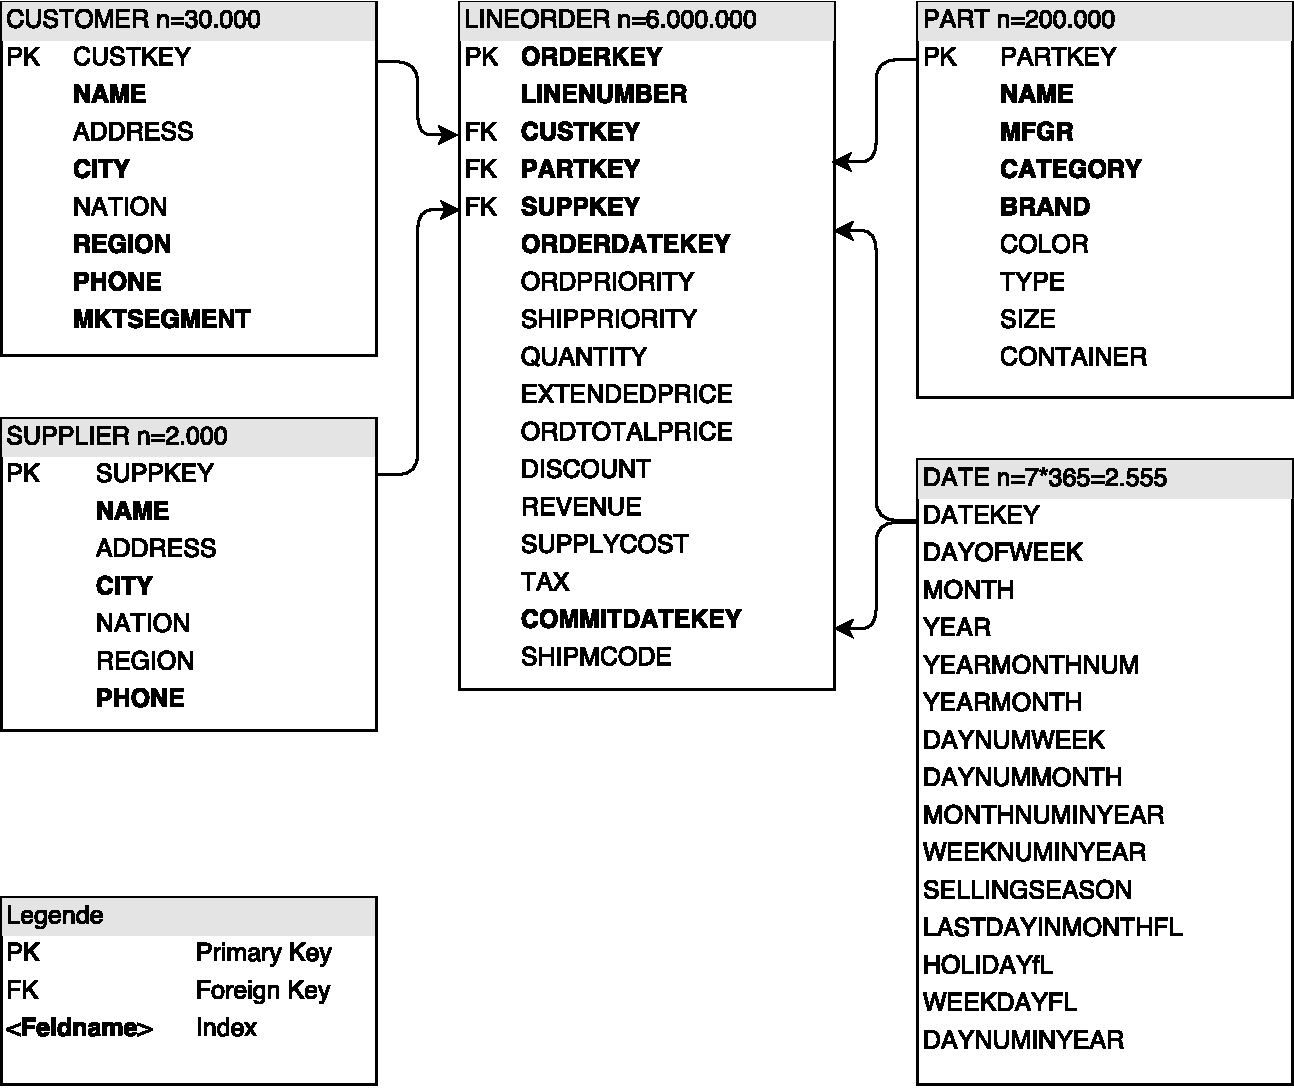
\includegraphics[scale=0.6]{ssbm_basic.pdf}}
\end{figure}  

Das genutze logische Schema des Benchmarks sieht folgende Tabellen vor: 
\begin{itemize}
	\item \textbf{{\glqq}COSTUMER{\grqq}}: Die Tabelle {\glqq}COSTUMER{\grqq} hat den Primärschlüssel {\glqq}CUSTKEY{\grqq} und umfasst 30 Tausend Datensätze. Indizes werden über die Felder {\glqq}NAME{\grqq}, {\glqq}CITY{\grqq}, {\glqq}REGION{\grqq}, {\glqq}PHONE{\grqq} und {\glqq}MKTSEGMENT{\grqq} gebildet. 
	\item \textbf{{\glqq}PART{\grqq}}: Die Tabelle {\glqq}PART{\grqq} enthält 200 Tausend Datensätze und hat den Primärschlüssel {\glqq}PARTKEY{\grqq}. Indizes werden über die Felder {\glqq}NAME{\grqq}, {\glqq}MFGR{\grqq}, {\glqq}CATEGORY{\grqq} und {\glqq}BRAND{\grqq} gebildet. 
	\item \textbf{{\glqq}SUPPLIER{\grqq}}: Die Tabelle {\glqq}SUPPLIER{\grqq} umfasst 2 Tausend Datensätze und hat den Primärschlüssel {\glqq}SUPPKEY{\grqq}. Indizes werden über die Felder {\glqq}NAME{\grqq}, {\glqq}CITY{\grqq} und {\glqq}PHONE{\grqq} gebildet. 
	\item \textbf{{\glqq}DATE{\grqq}}: Die Tabelle {\glqq}DATE{\grqq} hat den Primärschlüssel {\glqq}DATEKEY{\grqq} und hält 2,555 Tausend Einträge. Ihre Datensätze werden über {\glqq}ORDERDATEKEY{\grqq} und {\glqq}COMMITDATEKEY{\grqq} zugleich aggregiert. 
	\item \textbf{{\glqq}LINEORDER{\grqq}}: Die Tabelle {\glqq}LINEORDER{\grqq} hat den Primärschlüssel {\glqq}ORDERKEY{\grqq} und verweist über die Fremdschlüssel {\glqq}CUSTKEY{\grqq}, {\glqq}PARTKEY{\grqq}, {\glqq}ORDERDATEKEY{\grqq}, {\glqq}COMMITDATEKEY{\grqq} und {\glqq}SUPPKEY{\grqq} auf Datensätze der anderen Tabellen. Die Tabelle umfasst ca. 6 Millionen Einträge. Indizes werden über die Felder {\glqq}ORDERKEY, {\glqq}LINENUMBER, {\glqq}CUSTKEY{\grqq}, {\glqq}PARTKEY{\grqq}, {\glqq}SUPPKEY{\grqq}, {\glqq}ORDERDATEKEY{\grqq} und {\glqq}COMMITDATEKEY{\grqq} gebildet. 
\end{itemize}








	\chapter{Setup}
Diese Kapitel beschreibt das grundlegende Setup, um mit der SAP HANA Datenbank, in Form einer virtuellen Maschine, arbeiten zu können.

\section{Virtuelle Maschine}
Unter dem folgenden Link\footnote{\url{https://www.sap.com/developer/topics/sap-hana-express.html}}  kann eine SAP HANA Instanz heruntergeladen werden. Für den initialen Setup ist dieser URL\footnote{\url{https://www.sap.com/developer/tutorials/hxe-ua-getting-started-vm.html}}  notwendig und hilfreich.\\
Das Tutorial beschreibt dabei, wie eine SAP HANA Datenbank mithilfe einer Virtualisierungssoftware (z.B. VMware Player oder VirtualBox) realisiert wird. Um den Datenaustausch zwischen der virtuellen Maschine, und dem Host bequem zu gestalten ist es hilfreich, Daten die die VM benötigt entweder mit einem \enquote{Shared Folder} zu teilen, oder aber mit \enquote{Secure Copy} (SCP) in die VM zu übertragen.


\section{\enquote{Eclipse}}
Damit verschiedene Operationen auf der SAP HANA Datenbank ausgeführt werden können, ist es ratsam die Entwicklungsumgebung \enquote{Eclipse} zum Ausführen von SQL Statements zu nutzen. \\Unter dem folgenden Link\footnote{\url{https://www.sap.com/developer/how-tos/2016/09/hxe-howto-eclipse.html}} ist beschrieben, welche Erweiterungen und Einstellungen in \enquote{Eclipse} vorgenommen werden müssen, um eine Verbindung zur Datenbank herzustellen.

\subsection{Query Execution Plan}
Um nachvollziehen zu können, in welcher Abfolge die SQL Statements von der HANA Datenbank verarbeitet werden, lassen sich Query Execution Pläne erstellen.
Dafür sind folgende Schritte notwendig:
\begin{enumerate}
	\item SQL Console öffnen \& Statement eingeben
	\item \enquote{Rechtsklick} im Context Fenster der SQL Console
	\item Wähle den Menüpunkt \enquote{Visualize Plan} $\rightarrow$ \enquote{Execute} aus.
	\item Der Query Execution Plan wird nun angezeigt.
\end{enumerate} 

\section{Daten Import}
Dieser Abschnitt beschreibt, wie die SSBM-Benchmark-Daten in die SAP HANA Datenbank geladen werden können. Dies kann entweder über die SQL Console der Entwicklungsumgebung Eclipse geschehen, oder über die Kommandozeile der virtuellen Maschine, indem mittels \enquote{HDBSQL} die verschiedenen Dateien für das Anlegen des Schemas, den Import, etc. ausgeführt wird.
\\Um das Importieren möglichst einfach zu gestalten, ist es hilfreich die Daten als tbl- oder csv-Datei in einem beliebigen Verzeichnis in der virtuellen Maschine abzuspeichern.
\\Zu Beginn müssen die Tabellenschemata des SSBM-Benchmarks definiert werden. Dies passiert mit dem in \autoref{schema} dargestellten Statements. Begonnen wird der Benchmark, indem die Daten in einem Column Store gespeichert werden.\\
Um die Unterschiede zwischen Column und Row Store feststellen zu können, wird die Datenspeicherung pro Tabelle mithilfe der in \autoref{switchToRow} aufgezeigten SQL Statements von Column zu Row Store geändert. \\Außerdem ist in dem \autoref{switchToRow} zu erkennen, dass die Tabelle \enquote{Lineorder} zuerst gelöscht und neu erstellt wird. Dies hat als Grund, dass es Probleme gibt, falls die virtuelle Maschine zu wenig (< 8 GB) Arbeitsspeicher zugewiesen bekommt und somit den Befehl nicht erfolgreich abschließen kann. Zudem ist zu berücksichtigen, dass die Tabelle Lineorder mit Abstand am meisten Datensätze enthält.\\
Nachdem das Schema nun angelegt wurde, können nun die SSBM-Benchmark-Daten importiert werden. Das Importieren der Daten wird in \autoref{importSQL} Listing dargestellt. In diesem aktuellen Fall werden tbl-Daten für den Import genutzt. Es ist allerdings auch möglich die Daten über csv-Dateien in die Datenbank zu laden.



	\chapter{Ausführung des Benchmarks}

Das HANA Studio Plugin für Eclipse ermöglicht die direkte Ausführung von SQL-Code über die SQL-Console und würde damit ausreichen um die Schemata anzulegen, die Daten zu importieren und den Benchmark auszuführen. Werden nun jedoch Ansprüche wie das mehrfache Ausführen des Benchmarks unter unterschiedlichen Bedingungen gestellt, so ist offensichtlich, dass das händische Ausführen der einzelnen Schritte nachteilig ist. Eine elegantere Lösung ist die des Einsatzes von Skripten, welche Logik implementieren zur automatisierten Ausführung der Benchmarks. Dem Prozess der Ausführung des Benchmarks liegen dabei mehrere Gedanken zugrunde, welche in diesem Kapitel vorgestellt werden. 

\section{Ziele}

Die erwähnten Ansprüche an den kompletten Benchmark beziehen sich unter anderem auf seine \textbf{erleichtete Ausführung}. Wie im Kapitel zum Setup vorgestellt wurde, existiert ein Bash Skript {\glqq}run{\textunderscore}benchmark.bash{\grqq}, welches das zentrale Skript darstellt und dessen alleiniger Aufruf zur Ausführung des kompletten Benchmarks ausreicht. Somit ist die Komplexität der Ausführung für den Anwender reduziert. Nicht nur wird dadurch die Ausführung an sich erleichtert, auch die Installation des HANA Studio Plugins für Eclipse wird überflüssig, da jegliche SQL-Befehle automatisch über das Skript aus SQL-Dateien ausgeführt wird. Es sind also keine SQL-Kenntnisse für den Anwender notwendig, jeglich der Umgang mit Bash-Skripten. 

Die erleichterte Ausführung und Einrichtung der Benchmark-Umgebung ist es einfach den Benchmark auf \textbf{unterschiedlichen Test-Systemen} ausführen zu können. Durch die Variation der Test-Systeme können Faktoren wie die Anzahl zur Verfügung gestellter CPU Kerne oder RAM in ihrem Einfluss auf den Benchmark untersucht werden. Auf diese Aspekte wird im Folgekapitel näher eingegangen. 

Da die Evaluierung der Ergebnisse erst durchgeführt werden kann sobald alle Ergebnisse vorhanden sind (also nach Ausführung aller Benchmarks) muss eine Möglichkeit geschaffen werden, die Ergebnisse zwischenzuspeichern. Zu diesem Zwecke werden während der Durchführung der Benchmarks \textbf{Logs} angelegt, welche die Daten halten. 

Ein weiterer Aspekt ist die \textbf{Anzahl an Iterationen} innherhalb des kompletten Benchmarks. Viele Iterationen stellen den Ausschluss von Anomalien sicher und geben dem \textbf{Analyser} in der späteren Evaluierung zuverlässigere Werte. Dieser wird die Ergebnisse vergleichen und in einem einzigen Dokument erfassen. 

Nicht nur werden die Bedingungen für die Benchmarks variiert, sondern auch deren Inhalt. So werden unterschiedliche Konstellationen im Einsatz von \textbf{Row- und Columnstore} sowie \textbf{Indizes} durchgespielt. Genau wie die Variation des Test-Systems lassen sich dadurch essentielle Daten für den Analyser generieren. 

\section{Realisierung der Ziele}

Die eingesetzten Test-Systeme variieren folgendermassen: 
\begin{itemize}
	\item \textbf{RAM}: Es werden 6, 8 und 12 Gigabyte von 1.6 Tausend MHz DDR3 bis hin zu 3 Tausend MHz DDR4 RAM zur Verfügung gestellt. 
	\item \textbf{CPU}: Es werden 2, 4 und 6 virtuelle Kerne von 3.30GHz bis 4.2GHz zur Verfügung gestellt. 
\end{itemize}

Die Anzahl der Iterationen wird auf den Wert 250 festgelegt.

\newpage

\section{Durchführung}

\begin{wrapfigure}{r}{0.25\textwidth} 
    \centering{
    \includegraphics[scale=0.7]{images/Durchfuehrung3.png}
    \caption{Durchführung}\label{durchfuehrung}}
\end{wrapfigure}

Wie in \autoref{durchfuehrung} zu erkennen ist, lässt sich die Durchführung des Benchmarks unterteilen in die Schritte Schema Erzeugung, Daten Import, Index Erzeugung, Ausführung des Benchmarks, Speicherung der Daten ins Log und die Analyse durch den Analyser unterteilen. Zur Übersichtlichkeit wird ein simplifizierter Prozess dargestellt, denn die eigentliche Durchführung involviert mehrere Unterschritte, die die angesprochende inhaltliche Variation des Benchmarks realisieren. 

Nach erfolgreicher Anmeldung über die Zugangsdaten zur HANA Instanz erfolgt zuerst der Benchmark auf Basis eines Columnstores ohne Indizies. Dazu werden zuerst die Daten importiert und das Schema für den Columnstore angelegt. Anschliessend werden über den Aufruf des Skriptes {\glqq}all{\textunderscore}benchmarks.bash{\grqq} die einzelnen Queries ausgeführt. 

Nach der Ausführung des ersten Benchmarks werden in drei Schritten Indizes hinzugefügt und jeweils erneut Benchmarks durchgeführt. Darauf schliesst sich der Wechsel zum Rowstore an, was zuerst das Anlegen des Schemas für den Rowstore und ein erneutes Importieren der Daten involviert. Die Schritte zum Ausführen des Benchmarks bei unterschiedlichen Indizes werden nun wiederholt. 

Eine Iteration des Skriptes resultiert damit in acht einzelnen Benchmarks. Die Daten aus den Logs werden im folgenden Schritt vom Analyser analysiert. Die Auswertung des Benchmarks bezieht sich vorallem auf folgende System-Konfiguration: 6 Kerne @ 4.2GHz bei 8 Gigybyte RAM. 

	\chapter{Auswertung Benchmark}

\section{Gesamtlaufzeit des Benchmarks}\label{auswertung:generell}

%TODO ROW, COLUMN
% Grundlegende Statistische messwerte

\section{Vergleich Zeilenbasiert vs. Spaltenbasiert}\label{auswertung:row_vs_col}

%TODO
% Hypothese Spaltenbasiert ist schneller
% Welches is schneller
% Wie unterscheidet sich die Standardabweichung
% Bestätigung der Hypothese

\section{Einfluss der grundlegenden Indizes}\label{auswertung:basic_indizes}


	\chapter{Fazit}\label{chapter:fazit}
Generell lässt sich sagen, dass der Columnstore für die im SSBM Benchmark
geschaffenen Bedingungen deutlich besser geeignet ist.
In Zahlen bedeutet dies, dass der Columnstore im Schnitt mehr als 4 mal so schnell ist,
wie der Rowstore.

Die exemplarische Analyse der Query Execution Pläne für Query 4.3 hat gezeigt,
dass der große zeitliche Unterschied zwischen Row- und 
Columnstore darauf zurückzuführen ist, dass die Queries im Columnstore paralellisiert ablaufen.
Hier gibt es außerdem eine klare Trennung zwischen Filter und Join,
beim Rowstore ist dies enger miteinander verknüpft. 


Durch Indizes kann der Benchmark in beiden Fällen nochmals teils deutlich beschleunigt werden,
allerdings gibt es besonders beim Rowstore auch Fälle,
wo bestimmte Queries durch die Indizes verlangsamt wurden.
Indizes sollten also bewusst eingesetzt und auf ungewünschte Nebeneffekte geprüft werden.

Außerdem hat sich gezeigt, dass die optimierte OLAP-Engine deutlich schneller ist,
also die schnellste Variante der Column-Engine.
In der Praxis kann es von Vorteil sein, Abfragen als Analytical Views zu realisieren,
um diese Engine nutzen zu können. Für Rowstores ist die Engine leider nicht verfügbar.

Des Weiteren hat sich gezeigt, dass der Columnstore von mehr CPU-Kernen profitiert,
da hier sehr stark parallelisiert werden kann. 
Die Messwerte lassen auf einen quadratischen Zuwachs der Ausführungszeit
abhängig zur Anzahl der CPU-Kerne schliessen.
Durch reduzieren des Hauptspeicher nahm die Stabilität des Benchmarks stark ab,
was vermutlich darauf zurückzuführen ist, dass bei reduziertem RAM
externe Faktoren (Cache-Miss, Zugriffszeit) zum tragen kommen. 

Beim Rowstore hat sich gezeigt, dass hier sowohl CPU als auch RAM von größerer
Bedeutung für die Laufzeit sind. 
Während im Columnstore automatisch Optimierungen, wie Indexierung und Kompression stattfinden,
können diese im Rowstore womöglich nur bei ausreichend RAM durchgeführt werden. 

Zusammenfassend lässt sich sagen, dass die oft im Netz zu findende Empfehlung,
hauptsächlich auf Columnstores zu setzen, durch unsere Ergebnisse unterstützt wird.

	%Nur für Abgabe an der DHBW
	\chapter{Autoren - Wer hat was geschrieben}
\begin{table}[H]
    \centering
    \begin{tabularx}{\textwidth}{llX}
    \toprule
	Name                &	Matrikelnummer  & Hat geschrieben \\
    \toprule
    Jendrik Jordan      &                   & \\
    Arwed Mett          &                   & \\
    Simon Oswald        &   6594512         & \autoref{abstract},\autoref{auswertung:basic_indizes},\autoref{auswertung:olap},\autoref{chapter:fazit} \\
    Dominic Steinhauser &                   & \\
    \bottomrule
    \end{tabularx}
    \label{tab:autoren}
\end{table}
	%\chapter{Recherche}

Eine Datenbank hat die folgenden Performanz Faktoren\footnote{Vgl. \cite{sap:hana:performance_guide}[Seite 6]}:

\begin{itemize}
	\item Resourcen $\rightarrow$ CPU, Hauptspeicher, Festplatte
	\item Größe und Wachstum der Datenstrukturen
	\item Transaktionen
	\item Sicherheit, Autorisierung, und Lizensierung
	\item Konfiguration
\end{itemize}

\section{Permanent Langsames System}
Ein langsames System kann von vielen Faktoren abhängen.
Oft liegt es allerdings an zu wenigen Resourcen.
Dies kann mittels \verb+Administration > Overview+ oder \\
\verb+Administration > Performance > Load+ überprüft werden,
idem dort eine konstant hohe CPU, Hauptspeicher oder Netzwerk Auslastung angezeigt wird.

Dies kann auch mittels eines Betriebssystem Tools wie HTOP
analysiert werden.\footnote{Vgl. \cite{sap:hana:performance_guide}[Seite 8]}

% Wenn andere Queries laufen kann es sein dass HANA paging betreibt und ein Performanz test unnötig wäre.

%TODO Statement Performance Analysis

\section{Lizenzprobleme}
Es kann sein dass die Größe an speicher durch die Lizenz limitiert ist. (Siehe \cite{sap:hana:performance_guide}[Seite 9])

\section{Slow System-wide Performance}
Runtime Dump ausführen um zu analysieren.
\verb+\var\log\messages+ überprüfen um OS level Probleme zu erkennen.
\cite{sap:hana:performance_guide}[Seite 10]


\section{Hauptspeicher informationen}

\verb+Administration > Overview+
\verb+Configuration and Monitoring > Open Memory Overview+
Siehe \cite{sap:hana:performance_guide}[Seite 21]


%TODO Parallel Query execution
\cite{sap:hana:performance_guide}[Seite 40] $\rightarrow$ Parallele SQL Statement

%TODO IO

%TODO Delta Storage

%TODO Blocked Transaktionen

%TODO SQL Plan Cache Analysis

	
	\clearpage

	% Literaturverzeichnis
	\cleardoublepage
	\printbibliography

	% Glossar
	\printglossary[style=altlist,title=\langglossar]
	
	% sonstiger Anhang
	\clearpage
	\appendix
	% !TeX root = ../dokumentation.tex

\addchap{\langanhang}
\renewcommand{\thefigure}{A\arabic{figure}}

\setcounter{figure}{0}

\begin{lstlisting}[label=schemaCol, caption={Schema Columnstore}]
DROP TABLE  customer;

CREATE COLUMN TABLE  customer (
	C_CUSTOMERKEY INTEGER,
	C_Name varchar(25),
	C_Address varchar(25),
	C_City varchar(10),
	C_Nation varchar(15),
	C_Region varchar(12),
	C_Phone varchar(15),
	C_MktSegment varchar(10),
	PRIMARY KEY ("C_CUSTOMERKEY")
);

DROP TABLE  part;

CREATE COLUMN TABLE  part
(
	P_PartKey integer,
	P_Name varchar(25),
	P_MFGR varchar(10),
	P_Category varchar(10),
	P_Brand varchar(15),
	P_Colour varchar(15),
	P_Type varchar(25),
	P_Size tinyint,
	P_Container char(10),
	PRIMARY KEY (P_PartKey)
);



DROP TABLE  supplier;

CREATE COLUMN TABLE  supplier (
	S_SuppKey integer,
	S_Name char(25),
	S_Address varchar(25),
	S_City char(10),
	S_Nation char(15),
	S_Region char(12),
	S_Phone char(15),
	PRIMARY KEY(S_SuppKey)
);



DROP TABLE  dim_date;

CREATE COLUMN TABLE  dim_date
(
	D_DateKey integer,
	D_Date char(18),
	D_DayOfWeek char(9),
	D_Month char(9),
	D_Year smallint,
	D_YearMonthNum integer,
	D_YearMonth char(7),
	D_DayNumInWeek tinyint,
	D_DayNumInMonth tinyint,
	D_DayNumInYear smallint,
	D_MonthNumInYear tinyint,
	D_WeekNumInYear tinyint,
	D_SellingSeason char(12),
	D_LastDayInWeekFl tinyint,
	D_LastDayInMonthFl tinyint,
	D_HolidayFl tinyint,
	D_WeekDayFl tinyint,
	PRIMARY KEY(D_DateKey)
);

DROP TABLE lineorder;

CREATE COLUMN TABLE  lineorder
(
	LO_OrderKey bigint not null,
	LO_LineNumber tinyint not null,
	LO_CustKey int not null,
	LO_PartKey int not null,
	LO_SuppKey int not null,
	LO_OrderDateKey int not null,
	LO_OrderPriority varchar(15),
	LO_ShipPriority char(1),
	LO_Quantity tinyint,
	LO_ExtendedPrice decimal,
	LO_OrdTotalPrice decimal,
	LO_Discount decimal,
	LO_Revenue decimal,
	LO_SupplyCost decimal,
	LO_Tax tinyint,
	LO_CommitDateKey integer not null,
	LO_ShipMode varchar(10)
);
\end{lstlisting}

\begin{lstlisting}[label=schemaRow, caption={Schema Rowstore}]
DROP TABLE  customer;

CREATE ROW TABLE  customer (
	C_CUSTOMERKEY INTEGER,
	C_Name varchar(25),
	C_Address varchar(25),
	C_City varchar(10),
	C_Nation varchar(15),
	C_Region varchar(12),
	C_Phone varchar(15),
	C_MktSegment varchar(10),
	PRIMARY KEY ("C_CUSTOMERKEY")
);

DROP TABLE  part;

CREATE ROW TABLE  part
(
	P_PartKey integer,
	P_Name varchar(25),
	P_MFGR varchar(10),
	P_Category varchar(10),
	P_Brand varchar(15),
	P_Colour varchar(15),
	P_Type varchar(25),
	P_Size tinyint,
	P_Container char(10),
	PRIMARY KEY (P_PartKey)
);



DROP TABLE  supplier;

CREATE ROW TABLE  supplier (
	S_SuppKey integer,
	S_Name char(25),
	S_Address varchar(25),
	S_City char(10),
	S_Nation char(15),
	S_Region char(12),
	S_Phone char(15),
	PRIMARY KEY(S_SuppKey)
);



DROP TABLE  dim_date;

CREATE ROW TABLE  dim_date
(
	D_DateKey integer,
	D_Date char(18),
	D_DayOfWeek char(9),
	D_Month char(9),
	D_Year smallint,
	D_YearMonthNum integer,
	D_YearMonth char(7),
	D_DayNumInWeek tinyint,
	D_DayNumInMonth tinyint,
	D_DayNumInYear smallint,
	D_MonthNumInYear tinyint,
	D_WeekNumInYear tinyint,
	D_SellingSeason char(12),
	D_LastDayInWeekFl tinyint,
	D_LastDayInMonthFl tinyint,
	D_HolidayFl tinyint,
	D_WeekDayFl tinyint,
	PRIMARY KEY(D_DateKey)
);

DROP TABLE lineorder;

CREATE ROW TABLE  lineorder
(
	LO_OrderKey bigint not null,
	LO_LineNumber tinyint not null,
	LO_CustKey int not null,
	LO_PartKey int not null,
	LO_SuppKey int not null,
	LO_OrderDateKey int not null,
	LO_OrderPriority varchar(15),
	LO_ShipPriority char(1),
	LO_Quantity tinyint,
	LO_ExtendedPrice decimal,
	LO_OrdTotalPrice decimal,
	LO_Discount decimal,
	LO_Revenue decimal,
	LO_SupplyCost decimal,
	LO_Tax tinyint,
	LO_CommitDateKey integer not null,
	LO_ShipMode varchar(10)
);
\end{lstlisting}

\begin{lstlisting}[label=indizes, caption={Indizes hinzufügen}]
CREATE INDEX idx_c_name ON customer(C_Name);
CREATE INDEX idx_c_city ON customer(C_City);
CREATE INDEX idx_c_region ON customer(C_Region);
CREATE INDEX idx_c_phone ON customer(C_Phone);
CREATE INDEX idx_c_mktsegment ON customer(C_MktSegment);

CREATE INDEX idx_p_name ON part(P_Name);
CREATE INDEX idx_p_mfgr ON part(P_MFGR);
CREATE INDEX idx_p_category ON part(P_Category);
CREATE INDEX idx_p_brand ON part(P_Brand);

CREATE INDEX idx_s_city ON supplier(S_City);
CREATE INDEX idx_s_name ON supplier(S_Name);
CREATE INDEX idx_s_phone ON supplier(S_Phone);

CREATE INDEX idx_lo_orderkey_lo_linenumber ON lineorder(LO_OrderKey, LO_LineNumber);
CREATE INDEX idx_lo_custkey ON lineorder(LO_CustKey);
CREATE INDEX idx_lo_suppkey ON lineorder(LO_SuppKey);
CREATE INDEX idx_lo_partkey ON lineorder(LO_PartKey);
CREATE INDEX idx_lo_orderdatekey ON lineorder(LO_OrderDateKey);
CREATE INDEX idx_lo_commitdatekey ON lineorder(LO_CommitDateKey);
\end{lstlisting}




\begin{lstlisting}[label=importSQL, caption={import.sql}]
IMPORT FROM CSV FILE '/usr/sap/HXE/HDB90/work/date.tbl' INTO "SYSTEM"."DIM_DATE" 
WITH
record delimited by '\n' 
field delimited by '|';

IMPORT FROM CSV FILE '/usr/sap/HXE/HDB90/work/customer.tbl' INTO "SYSTEM"."CUSTOMER" 
WITH
record delimited by '\n' 
field delimited by '|';

IMPORT FROM CSV FILE '/usr/sap/HXE/HDB90/work/lineorder.tbl' INTO "SYSTEM"."LINEORDER" 
WITH
batch 10000
record delimited by '\n' 
field delimited by '|';

IMPORT FROM CSV FILE '/usr/sap/HXE/HDB90/work/part.tbl' INTO "SYSTEM"."PART" 
WITH
record delimited by '\n' 
field delimited by '|';

IMPORT FROM CSV FILE '/usr/sap/HXE/HDB90/work/supplier.tbl' INTO "SYSTEM"."SUPPLIER" 
WITH
record delimited by '\n' 
field delimited by '|';
\end{lstlisting}


\begin{figure}[H]
	\centering
	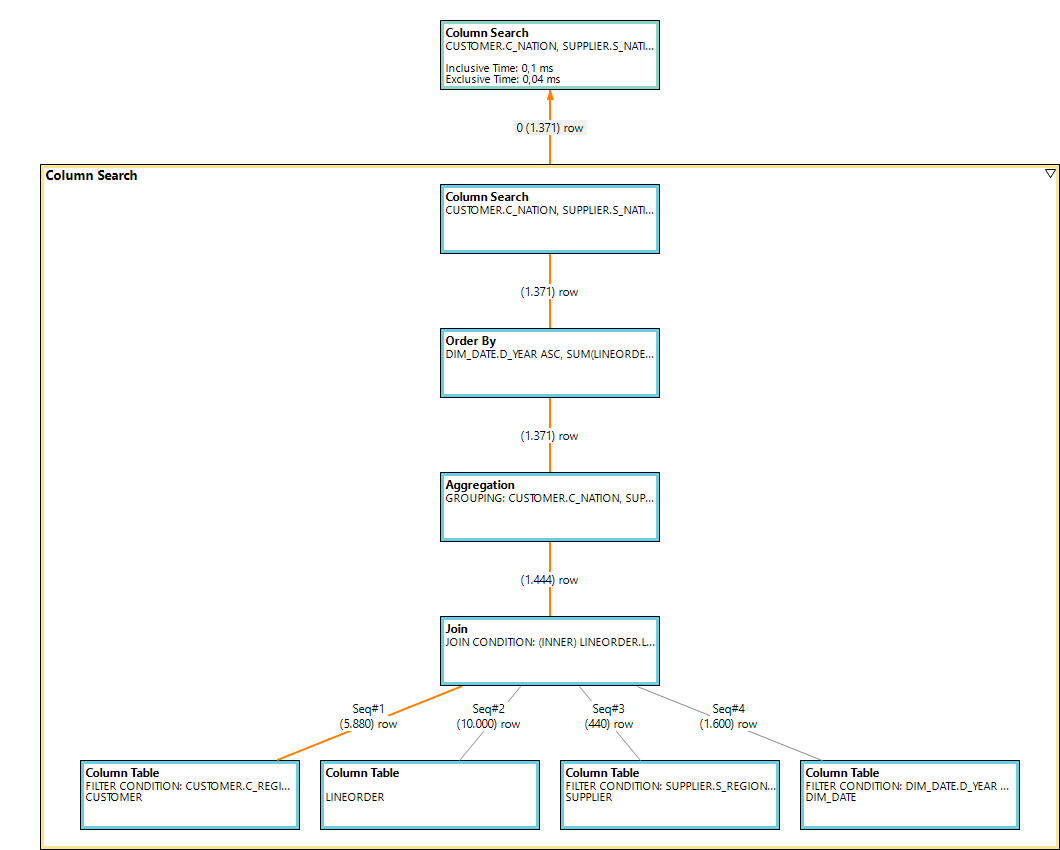
\includegraphics[width=0.7\textwidth]{images/q3-1-col-exec.png}
	\caption{Q3.1 Execution Plan - Comlumn Store}\label{auswertung:q3.1:col}
\end{figure}
\begin{figure}[H]
	\centering
	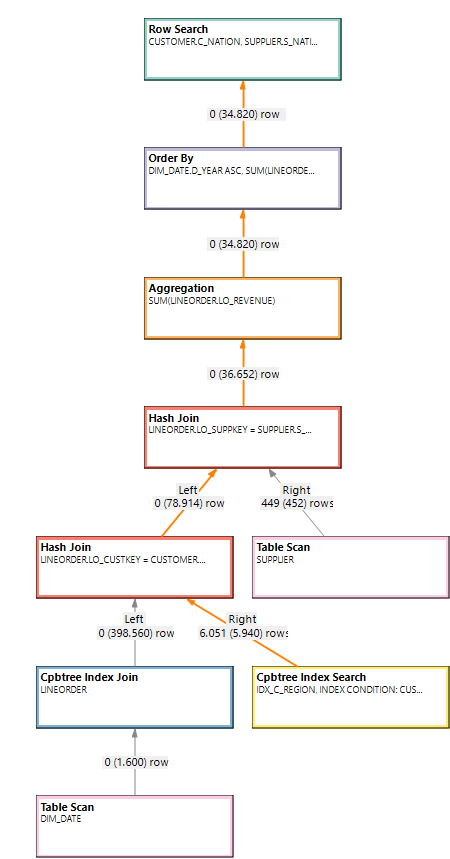
\includegraphics[width=0.7\textwidth]{images/q3-1-row-exec.png}
	\caption{Q3.1 Execution Plan - Rowstore}\label{auswertung:q3.1:row}
\end{figure}
\begin{figure}[H]
	\centering
	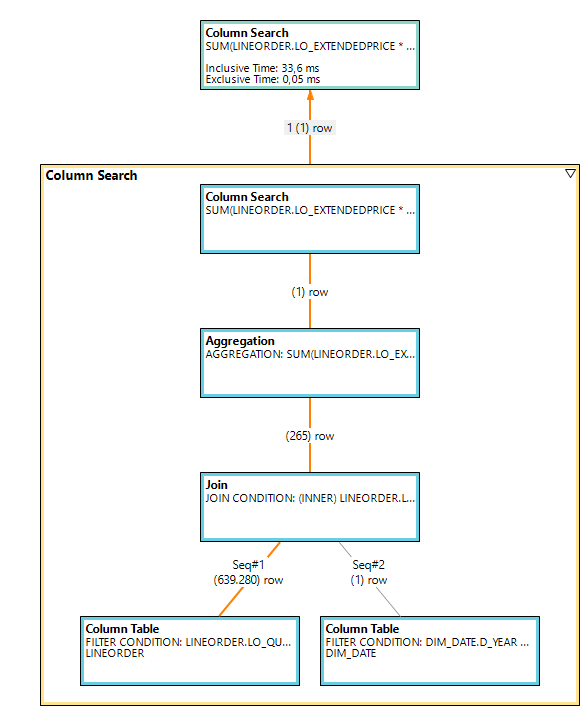
\includegraphics[width=0.7\textwidth]{images/q1-1-col-exec.png}
	\caption{Q1.1 Execution Plan - Columnstore}\label{exec:q1.1-col}
\end{figure}
\begin{figure}[H]
	\centering
	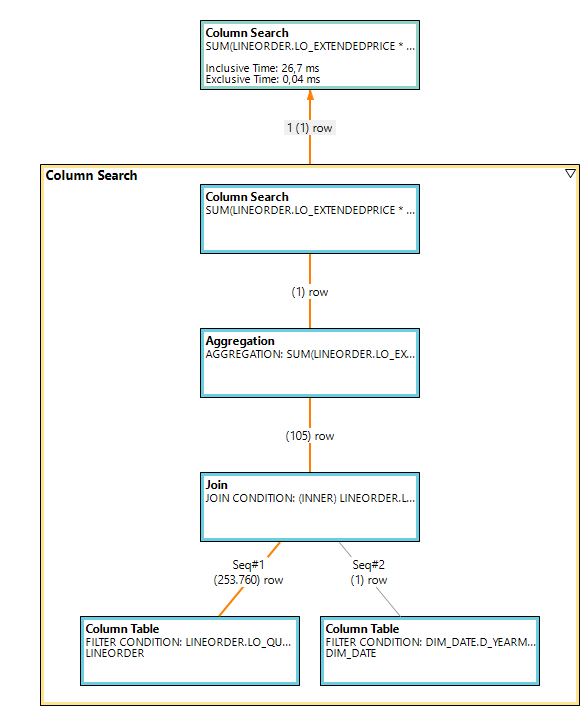
\includegraphics[width=0.7\textwidth]{images/q1-2-col-exec.png}
	\caption{Q1.2 Execution Plan - Columnstore}\label{exec:q1.2-col}
\end{figure}
\begin{figure}[H]
	\centering
	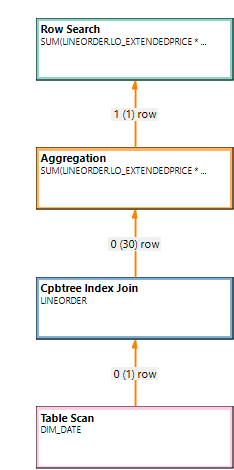
\includegraphics[width=0.7\textwidth]{images/q1-1-row-exec.png}
	\caption{Q1.1 Execution Plan - Rowstore}\label{exec:q1.1-row}
\end{figure}
\begin{figure}[H]
	\centering
	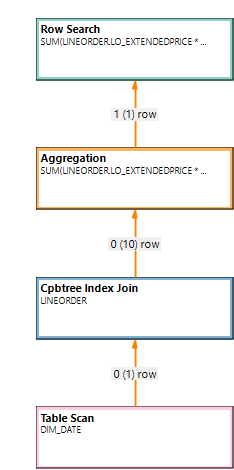
\includegraphics[width=0.7\textwidth]{images/q1-2-row-exec.png}
	\caption{Q1.2 Execution Plan - Rowstore}\label{exec:q1.2-row}
\end{figure}


\begin{figure}[H]
	\centering
	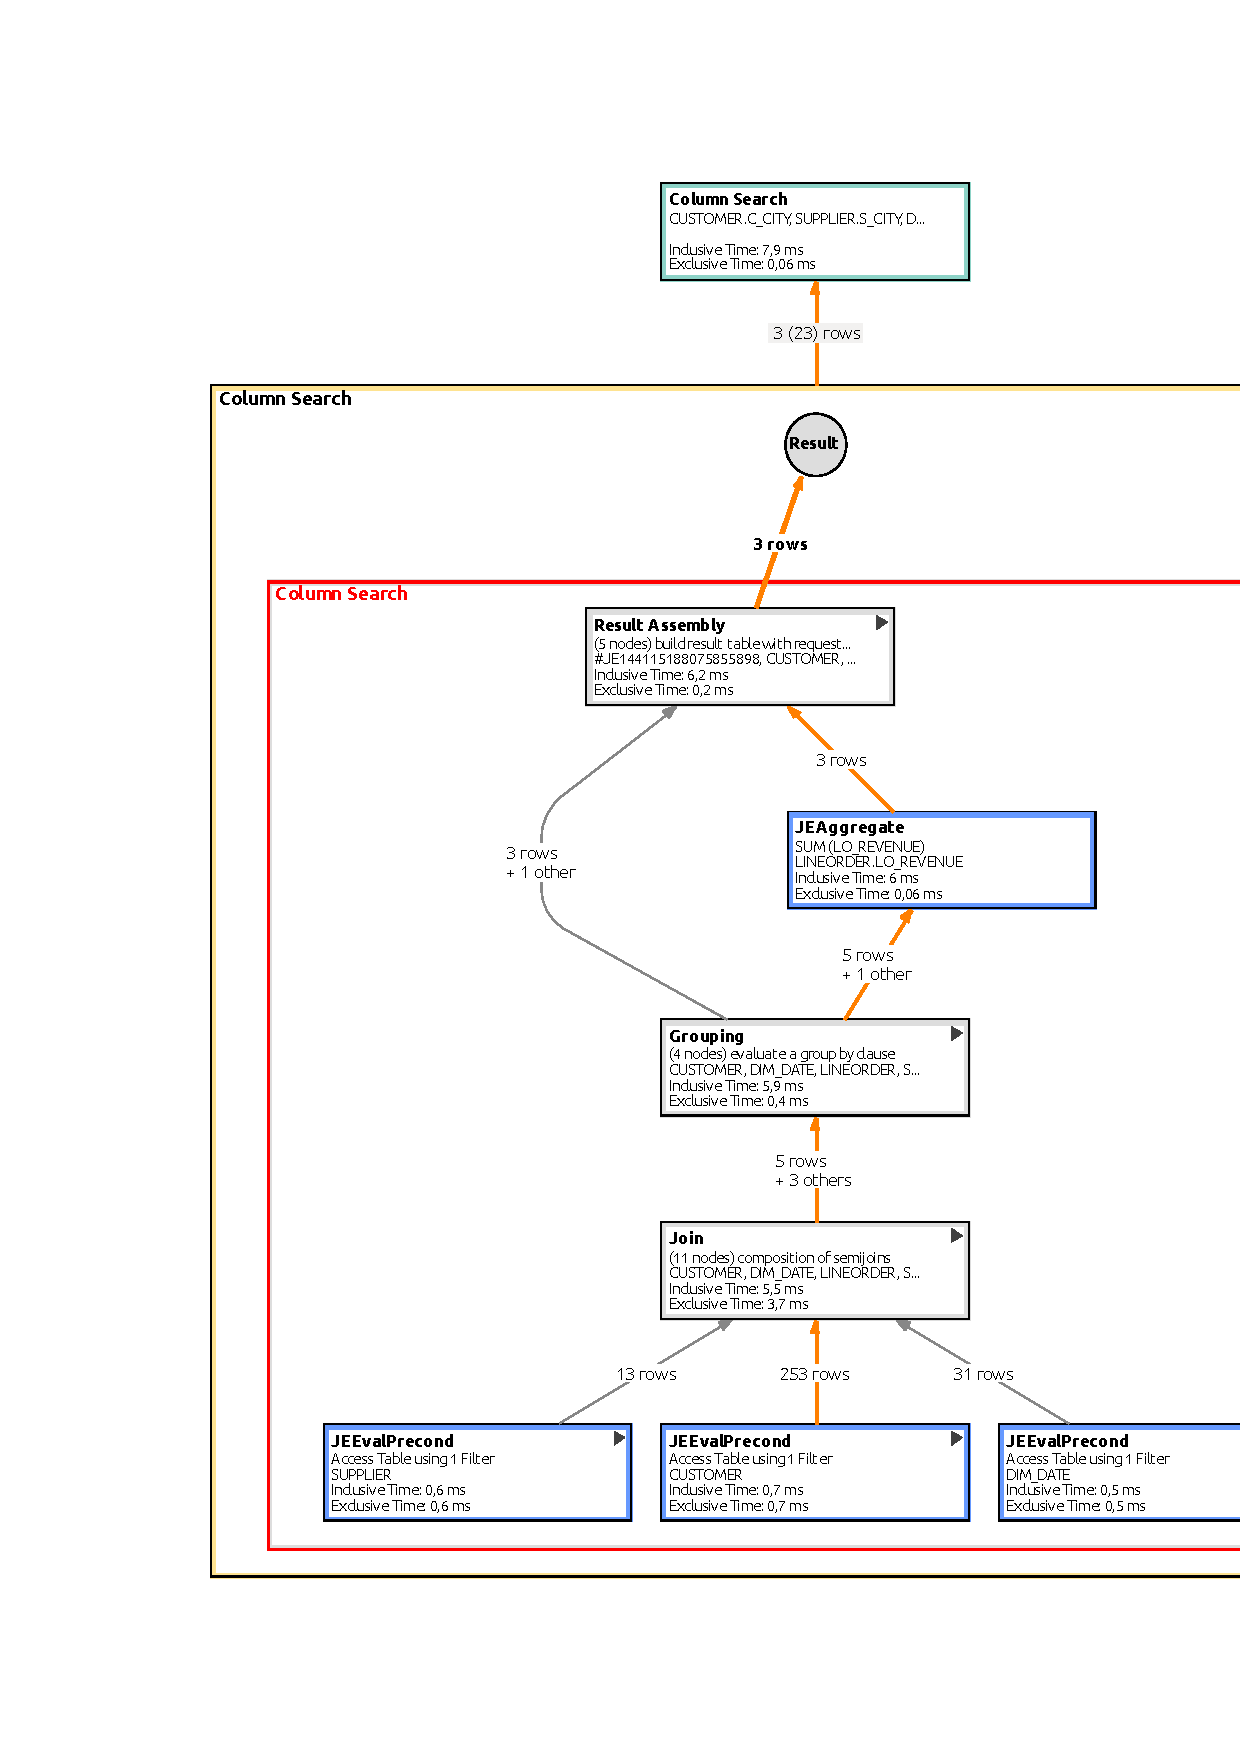
\includegraphics[width=\textwidth]{images/col_q34_index.pdf}
	\caption{Q3.4 Execution Plan - Columnstore mit Indizes}\label{exec:q34-col-index}
\end{figure}

\begin{figure}[H]
	\centering
	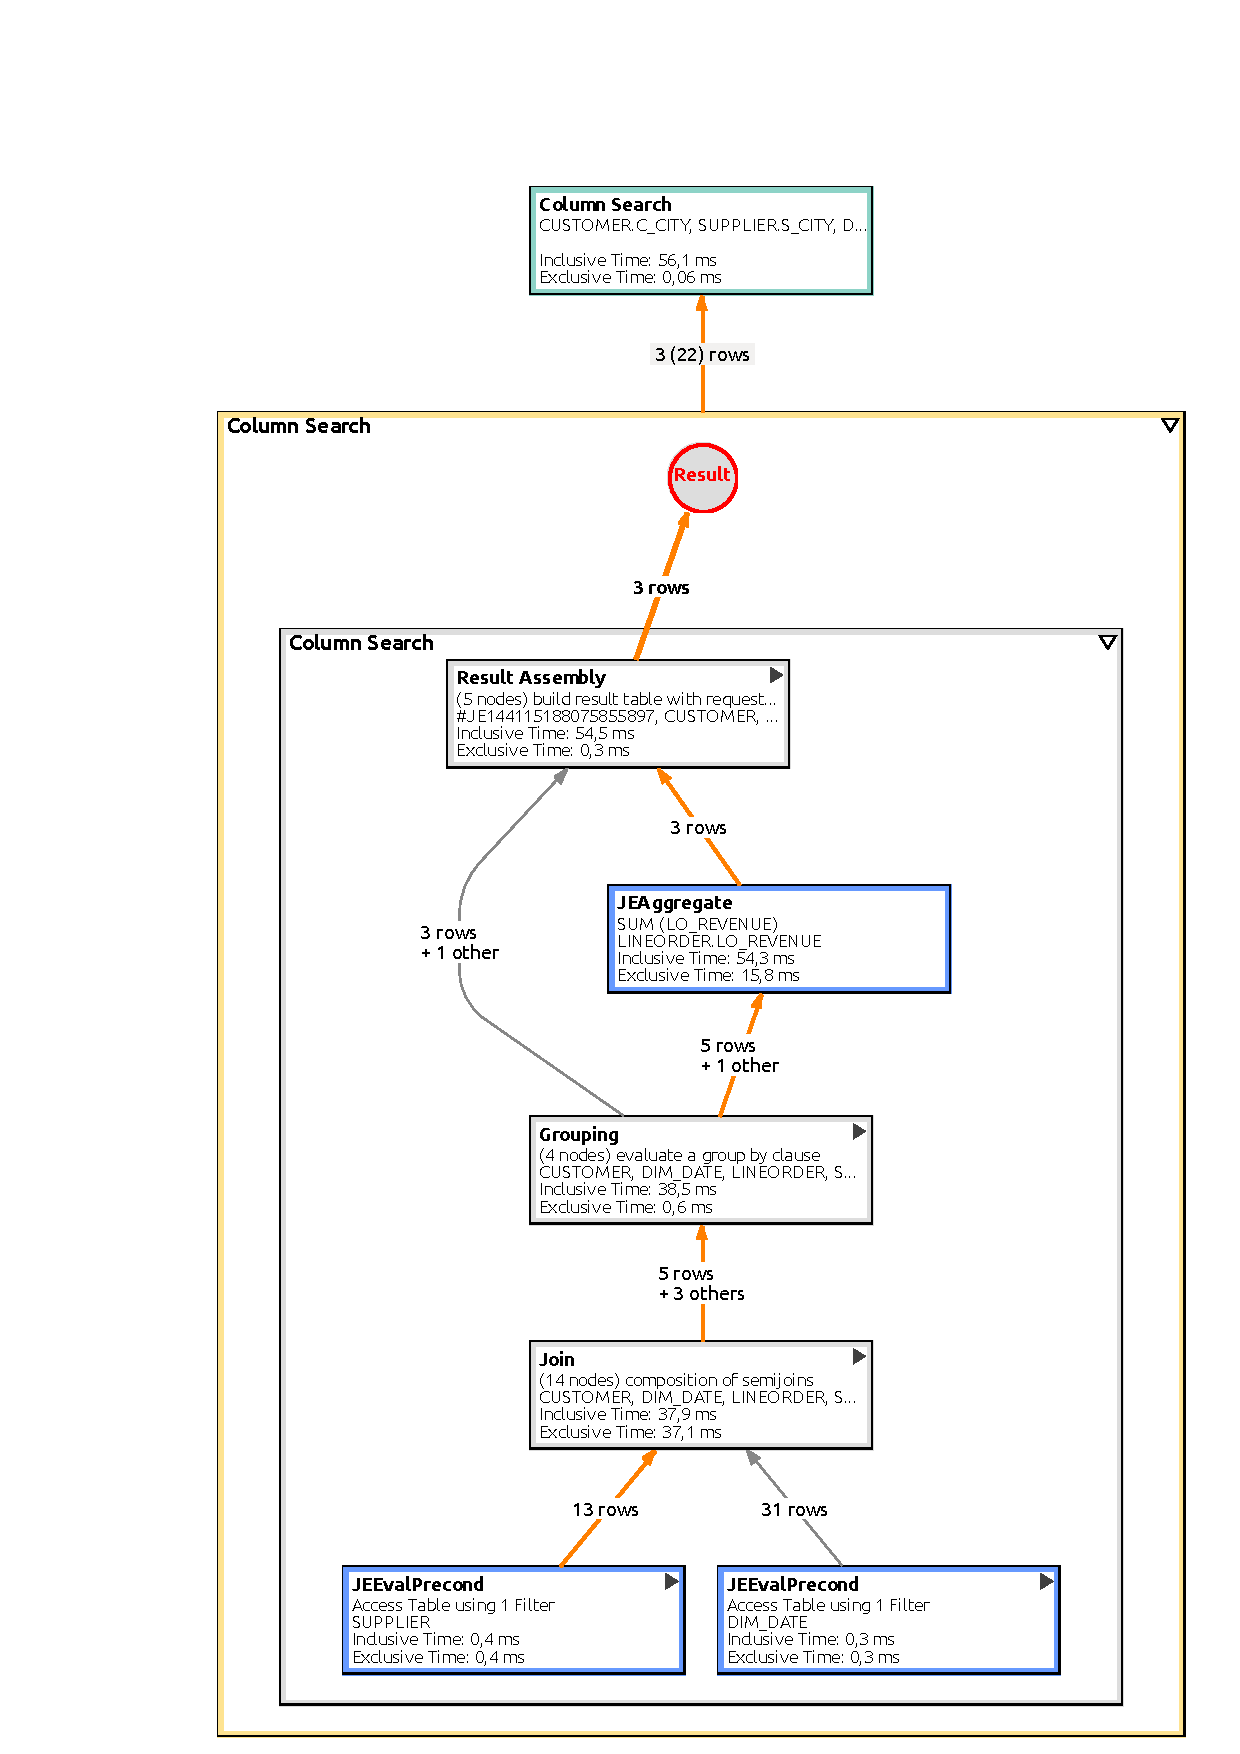
\includegraphics[width=\textwidth]{images/col_q34_no.pdf}
	\caption{Q3.4 Execution Plan - Columnstore ohne Indizes}\label{exec:q3.4-col-no}
\end{figure}

\begin{landscape}
	\begin{figure}[H]
		\centering
		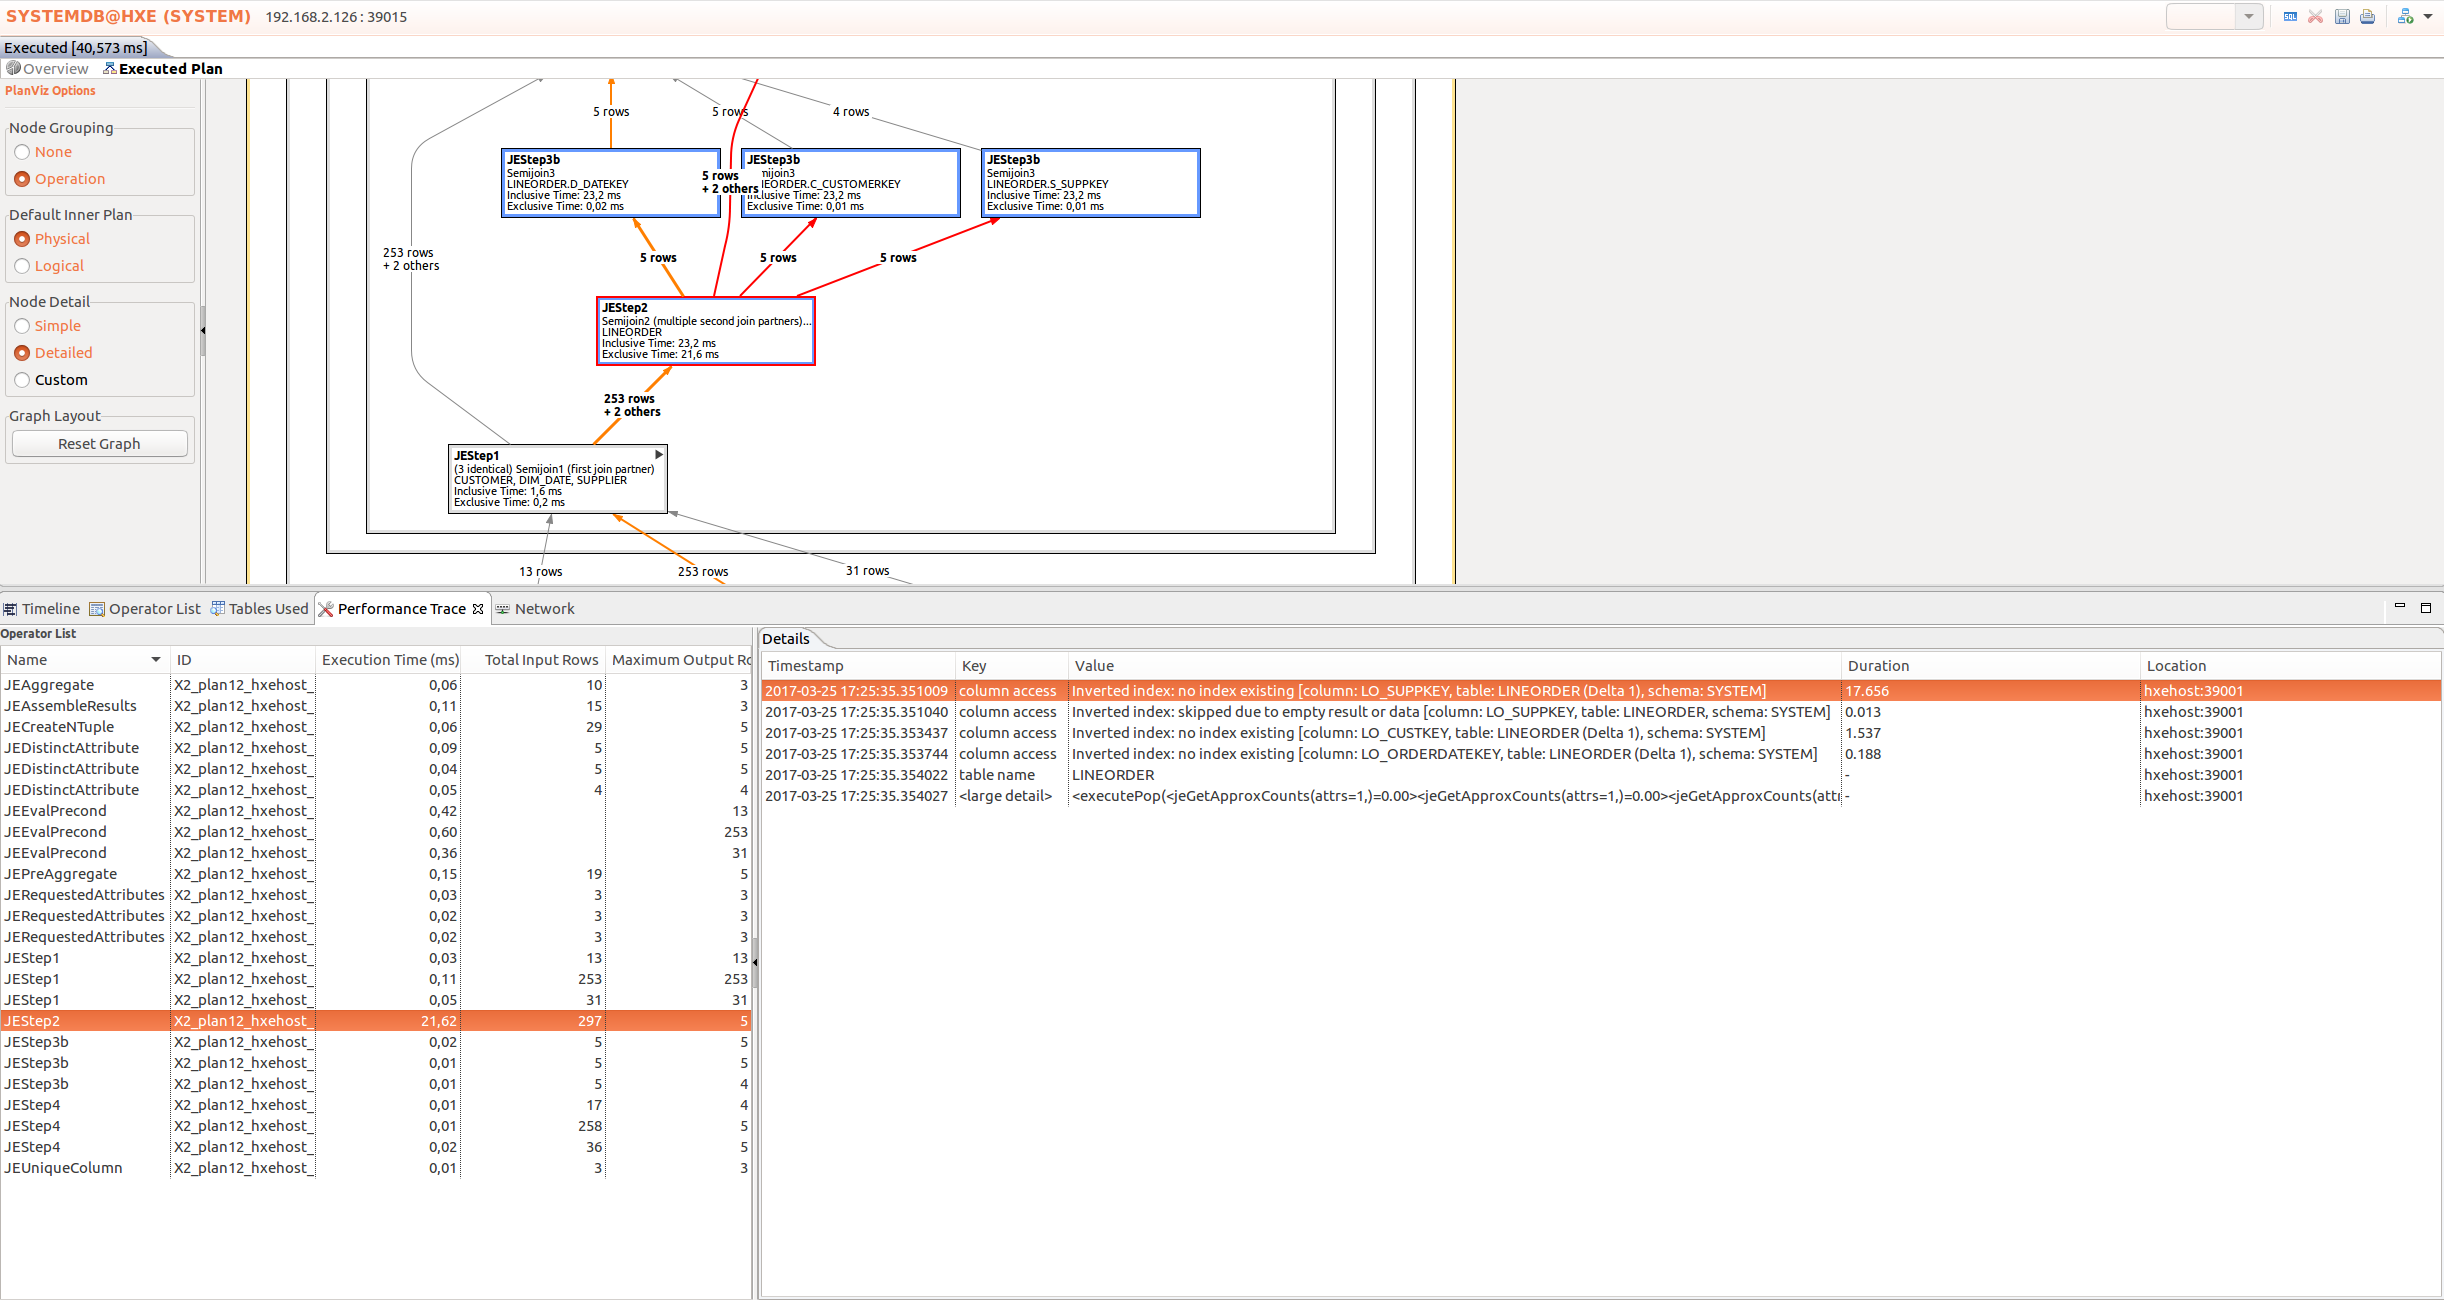
\includegraphics[scale=0.28]{images/execCol.png}
		\caption{Execution Plan: Q3.4}\label{execution-plan:before-index}
	\end{figure}
\end{landscape}
\begin{landscape}
	\begin{figure}[H]
		\centering
		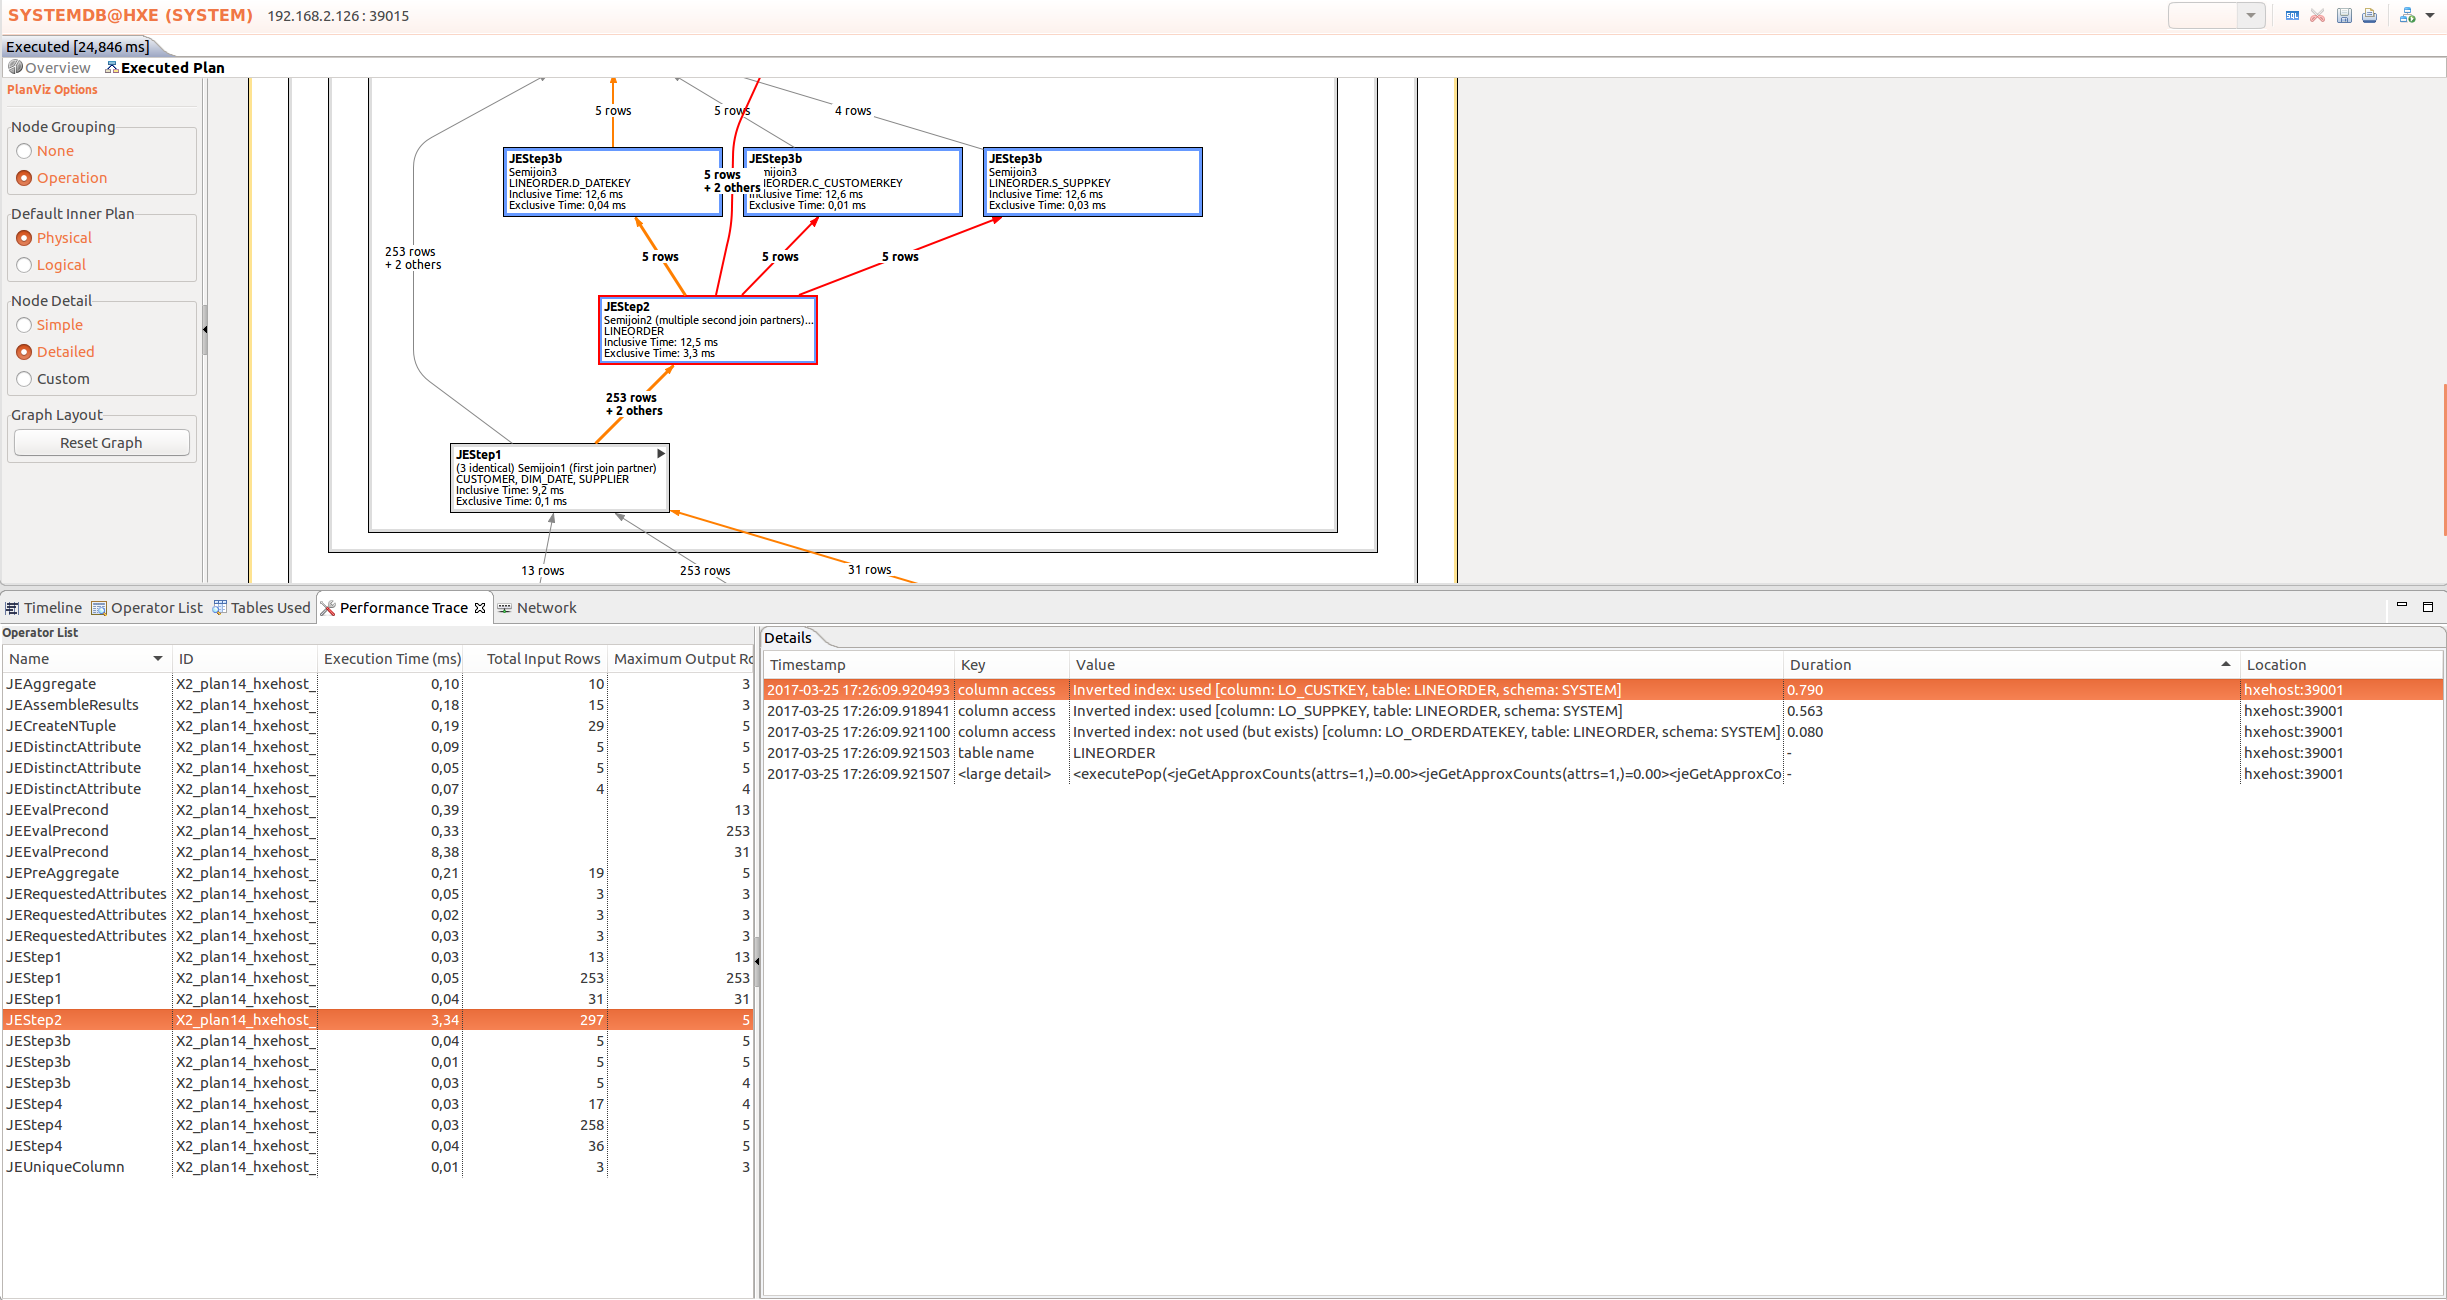
\includegraphics[scale=0.28]{images/execColIndex.png}
		\caption{Execution Plan: Q3.4 with Index}\label{execution-plan:after-index}
	\end{figure}
\end{landscape}

	
\end{document}
